\documentclass[aspectratio=43]{beamer}
\usetheme[
  block=fill,
  background=light,
  titleformat=smallcaps,
  progressbar=frametitle,
  %% numbering=none,
]{metropolis}
\setbeamersize{text margin left=.5cm,text margin right=.5cm}

%%%%%%%%%%%%%%%%%%%%%%%%%%%%%%%%%%%%%%%%%%
%% Packages
%%%%%%%%%%%%%%%%%%%%%%%%%%%%%%%%%%%%%%%%%%

% Colors
\usepackage{xcolor}

% Images
\usepackage{graphics}
\graphicspath{{img/}}

% Math Symbols
\usepackage{stmaryrd}

% Quotes
\usepackage{epigraph}

%%%%%%%%%%%%%%%%%%%%%%%%%%%%%%%%%%%%%%%%%%
%% Macros
%%%%%%%%%%%%%%%%%%%%%%%%%%%%%%%%%%%%%%%%%%
\renewcommand\alert[1]{\textcolor{mLightBrown}{#1}}

%%%%%%%%%%%%%%%%%%%%%%%%%%%%%%%%%%%%%%%%%%
%% Haskell imports
%%%%%%%%%%%%%%%%%%%%%%%%%%%%%%%%%%%%%%%%%%

%% ODER: format ==         = "\mathrel{==}"
%% ODER: format /=         = "\neq "
%
%
\makeatletter
\@ifundefined{lhs2tex.lhs2tex.sty.read}%
  {\@namedef{lhs2tex.lhs2tex.sty.read}{}%
   \newcommand\SkipToFmtEnd{}%
   \newcommand\EndFmtInput{}%
   \long\def\SkipToFmtEnd#1\EndFmtInput{}%
  }\SkipToFmtEnd

\newcommand\ReadOnlyOnce[1]{\@ifundefined{#1}{\@namedef{#1}{}}\SkipToFmtEnd}
\usepackage{amstext}
\usepackage{amssymb}
\usepackage{stmaryrd}
\DeclareFontFamily{OT1}{cmtex}{}
\DeclareFontShape{OT1}{cmtex}{m}{n}
  {<5><6><7><8>cmtex8
   <9>cmtex9
   <10><10.95><12><14.4><17.28><20.74><24.88>cmtex10}{}
\DeclareFontShape{OT1}{cmtex}{m}{it}
  {<-> ssub * cmtt/m/it}{}
\newcommand{\texfamily}{\fontfamily{cmtex}\selectfont}
\DeclareFontShape{OT1}{cmtt}{bx}{n}
  {<5><6><7><8>cmtt8
   <9>cmbtt9
   <10><10.95><12><14.4><17.28><20.74><24.88>cmbtt10}{}
\DeclareFontShape{OT1}{cmtex}{bx}{n}
  {<-> ssub * cmtt/bx/n}{}
\newcommand{\tex}[1]{\text{\texfamily#1}}	% NEU

\newcommand{\Sp}{\hskip.33334em\relax}


\newcommand{\Conid}[1]{\mathit{#1}}
\newcommand{\Varid}[1]{\mathit{#1}}
\newcommand{\anonymous}{\kern0.06em \vbox{\hrule\@width.5em}}
\newcommand{\plus}{\mathbin{+\!\!\!+}}
\newcommand{\bind}{\mathbin{>\!\!\!>\mkern-6.7mu=}}
\newcommand{\rbind}{\mathbin{=\mkern-6.7mu<\!\!\!<}}% suggested by Neil Mitchell
\newcommand{\sequ}{\mathbin{>\!\!\!>}}
\renewcommand{\leq}{\leqslant}
\renewcommand{\geq}{\geqslant}
\usepackage{polytable}

%mathindent has to be defined
\@ifundefined{mathindent}%
  {\newdimen\mathindent\mathindent\leftmargini}%
  {}%

\def\resethooks{%
  \global\let\SaveRestoreHook\empty
  \global\let\ColumnHook\empty}
\newcommand*{\savecolumns}[1][default]%
  {\g@addto@macro\SaveRestoreHook{\savecolumns[#1]}}
\newcommand*{\restorecolumns}[1][default]%
  {\g@addto@macro\SaveRestoreHook{\restorecolumns[#1]}}
\newcommand*{\aligncolumn}[2]%
  {\g@addto@macro\ColumnHook{\column{#1}{#2}}}

\resethooks

\newcommand{\onelinecommentchars}{\quad-{}- }
\newcommand{\commentbeginchars}{\enskip\{-}
\newcommand{\commentendchars}{-\}\enskip}

\newcommand{\visiblecomments}{%
  \let\onelinecomment=\onelinecommentchars
  \let\commentbegin=\commentbeginchars
  \let\commentend=\commentendchars}

\newcommand{\invisiblecomments}{%
  \let\onelinecomment=\empty
  \let\commentbegin=\empty
  \let\commentend=\empty}

\visiblecomments

\newlength{\blanklineskip}
\setlength{\blanklineskip}{0.66084ex}

\newcommand{\hsindent}[1]{\quad}% default is fixed indentation
\let\hspre\empty
\let\hspost\empty
\newcommand{\NB}{\textbf{NB}}
\newcommand{\Todo}[1]{$\langle$\textbf{To do:}~#1$\rangle$}

\EndFmtInput
\makeatother
%
%
%
%
%
%
% This package provides two environments suitable to take the place
% of hscode, called "plainhscode" and "arrayhscode". 
%
% The plain environment surrounds each code block by vertical space,
% and it uses \abovedisplayskip and \belowdisplayskip to get spacing
% similar to formulas. Note that if these dimensions are changed,
% the spacing around displayed math formulas changes as well.
% All code is indented using \leftskip.
%
% Changed 19.08.2004 to reflect changes in colorcode. Should work with
% CodeGroup.sty.
%
\ReadOnlyOnce{polycode.fmt}%
\makeatletter

\newcommand{\hsnewpar}[1]%
  {{\parskip=0pt\parindent=0pt\par\vskip #1\noindent}}

% can be used, for instance, to redefine the code size, by setting the
% command to \small or something alike
\newcommand{\hscodestyle}{}

% The command \sethscode can be used to switch the code formatting
% behaviour by mapping the hscode environment in the subst directive
% to a new LaTeX environment.

\newcommand{\sethscode}[1]%
  {\expandafter\let\expandafter\hscode\csname #1\endcsname
   \expandafter\let\expandafter\endhscode\csname end#1\endcsname}

% "compatibility" mode restores the non-polycode.fmt layout.

\newenvironment{compathscode}%
  {\par\noindent
   \advance\leftskip\mathindent
   \hscodestyle
   \let\\=\@normalcr
   \let\hspre\(\let\hspost\)%
   \pboxed}%
  {\endpboxed\)%
   \par\noindent
   \ignorespacesafterend}

\newcommand{\compaths}{\sethscode{compathscode}}

% "plain" mode is the proposed default.
% It should now work with \centering.
% This required some changes. The old version
% is still available for reference as oldplainhscode.

\newenvironment{plainhscode}%
  {\hsnewpar\abovedisplayskip
   \advance\leftskip\mathindent
   \hscodestyle
   \let\hspre\(\let\hspost\)%
   \pboxed}%
  {\endpboxed%
   \hsnewpar\belowdisplayskip
   \ignorespacesafterend}

\newenvironment{oldplainhscode}%
  {\hsnewpar\abovedisplayskip
   \advance\leftskip\mathindent
   \hscodestyle
   \let\\=\@normalcr
   \(\pboxed}%
  {\endpboxed\)%
   \hsnewpar\belowdisplayskip
   \ignorespacesafterend}

% Here, we make plainhscode the default environment.

\newcommand{\plainhs}{\sethscode{plainhscode}}
\newcommand{\oldplainhs}{\sethscode{oldplainhscode}}
\plainhs

% The arrayhscode is like plain, but makes use of polytable's
% parray environment which disallows page breaks in code blocks.

\newenvironment{arrayhscode}%
  {\hsnewpar\abovedisplayskip
   \advance\leftskip\mathindent
   \hscodestyle
   \let\\=\@normalcr
   \(\parray}%
  {\endparray\)%
   \hsnewpar\belowdisplayskip
   \ignorespacesafterend}

\newcommand{\arrayhs}{\sethscode{arrayhscode}}

% The mathhscode environment also makes use of polytable's parray 
% environment. It is supposed to be used only inside math mode 
% (I used it to typeset the type rules in my thesis).

\newenvironment{mathhscode}%
  {\parray}{\endparray}

\newcommand{\mathhs}{\sethscode{mathhscode}}

% texths is similar to mathhs, but works in text mode.

\newenvironment{texthscode}%
  {\(\parray}{\endparray\)}

\newcommand{\texths}{\sethscode{texthscode}}

% The framed environment places code in a framed box.

\def\codeframewidth{\arrayrulewidth}
\RequirePackage{calc}

\newenvironment{framedhscode}%
  {\parskip=\abovedisplayskip\par\noindent
   \hscodestyle
   \arrayrulewidth=\codeframewidth
   \tabular{@{}|p{\linewidth-2\arraycolsep-2\arrayrulewidth-2pt}|@{}}%
   \hline\framedhslinecorrect\\{-1.5ex}%
   \let\endoflinesave=\\
   \let\\=\@normalcr
   \(\pboxed}%
  {\endpboxed\)%
   \framedhslinecorrect\endoflinesave{.5ex}\hline
   \endtabular
   \parskip=\belowdisplayskip\par\noindent
   \ignorespacesafterend}

\newcommand{\framedhslinecorrect}[2]%
  {#1[#2]}

\newcommand{\framedhs}{\sethscode{framedhscode}}

% The inlinehscode environment is an experimental environment
% that can be used to typeset displayed code inline.

\newenvironment{inlinehscode}%
  {\(\def\column##1##2{}%
   \let\>\undefined\let\<\undefined\let\\\undefined
   \newcommand\>[1][]{}\newcommand\<[1][]{}\newcommand\\[1][]{}%
   \def\fromto##1##2##3{##3}%
   \def\nextline{}}{\) }%

\newcommand{\inlinehs}{\sethscode{inlinehscode}}

% The joincode environment is a separate environment that
% can be used to surround and thereby connect multiple code
% blocks.

\newenvironment{joincode}%
  {\let\orighscode=\hscode
   \let\origendhscode=\endhscode
   \def\endhscode{\def\hscode{\endgroup\def\@currenvir{hscode}\\}\begingroup}
   %\let\SaveRestoreHook=\empty
   %\let\ColumnHook=\empty
   %\let\resethooks=\empty
   \orighscode\def\hscode{\endgroup\def\@currenvir{hscode}}}%
  {\origendhscode
   \global\let\hscode=\orighscode
   \global\let\endhscode=\origendhscode}%

\makeatother
\EndFmtInput
%
%%%%%%%%%%%%%%%%%%%%%%%%%%%%%%
%%
%% Haskell Styling

\newenvironment{hs}
{}
{}

%% Colors (from duo-tone light syntax)
\definecolor{hsblack}{RGB}{45,32,3}
\definecolor{hsgold1}{RGB}{179,169,149}
\definecolor{hsgold2}{RGB}{177,149,90}
\definecolor{hsgold3}{RGB}{190,106,13}%{192,96,4}%{132,97,19}
\definecolor{hsblue1}{RGB}{173,176,182}
\definecolor{hsblue2}{RGB}{113,142,205}
\definecolor{hsblue3}{RGB}{0,33,132}
\definecolor{hsblue4}{RGB}{97,108,132}
\definecolor{hsblue5}{RGB}{34,50,68}
\definecolor{hsred2}{RGB}{191,121,103}
\definecolor{hsred3}{RGB}{171,72,46}

%% LaTeX Kerning nastiness. By using curly braces to delimit color group,
%% it breaks spacing. The following seems to work:
%%
%% https://tex.stackexchange.com/questions/85033/colored-symbols/85035#85035
%%
\newcommand*{\mathcolor}{}
\def\mathcolor#1#{\mathcoloraux{#1}}
\newcommand*{\mathcoloraux}[3]{%
  \protect\leavevmode
  \begingroup
    \color#1{#2}#3%
  \endgroup
}


\newcommand{\HSKeyword}[1]{\mathcolor{hsgold3}{\textbf{#1}}}
\newcommand{\HSNumeral}[1]{\mathcolor{hsred3}{#1}}
\newcommand{\HSChar}[1]{\mathcolor{hsred2}{#1}}
\newcommand{\HSString}[1]{\mathcolor{hsred2}{#1}}
\newcommand{\HSSpecial}[1]{\mathcolor{hsblue4}{\ensuremath{#1}}}
\newcommand{\HSSym}[1]{\mathcolor{hsblue4}{\ensuremath{#1}}}
\newcommand{\HSCon}[1]{\mathcolor{hsblue3}{#1}}
\newcommand{\HSVar}[1]{\mathcolor{hsblue5}{\mathit{\ensuremath{#1}}}}
\newcommand{\HSComment}[1]{\mathcolor{hsgold2}{\textit{#1}}}



%%% lhs2TeX parser does not recognize '*'
%%% in kind annotations, it thinks it is a multiplication.




%%% Datatype Promotion
%%format (P (a)) = "\HSSym{''}" a

%%% Usefull Notation



\def\commentbegin{}
\def\commentend{}


%%%%%%%%%%%%%%%%%%%%%%%%%%%%%%%%%%%%%%%%%%
%% Fonts
%%%%%%%%%%%%%%%%%%%%%%%%%%%%%%%%%%%%%%%%%%
\usepackage{relsize}
\usepackage[tt=false]{libertine}
\usepackage[libertine]{newtxmath}

%----------------------------------------------------------------------------

\title{Music as Language}
\subtitle{Putting Probabilistic Temporal Graph Grammars to Good Use}
\author{Orestis Melkonian}
\date{August 23, 2019}
\institute{Utrecht University, The Netherlands}

\begin{document}
\begin{center}
\maketitle
\end{center}

\section{Introduction}

\begin{frame}{Motivation}
\begin{itemize}
\item The aim is not to generate a complete music piece
  \begin{itemize}
  \item Rather an aid in the compositional process
  \end{itemize}
\item Do this in a concise way, which is also expressive enough
  \begin{itemize}
  \item To that end, we use formal grammars
  \end{itemize}
\end{itemize}
\end{frame}

\begin{frame}{Probabilistic Temporal Graph Grammars}
\centering
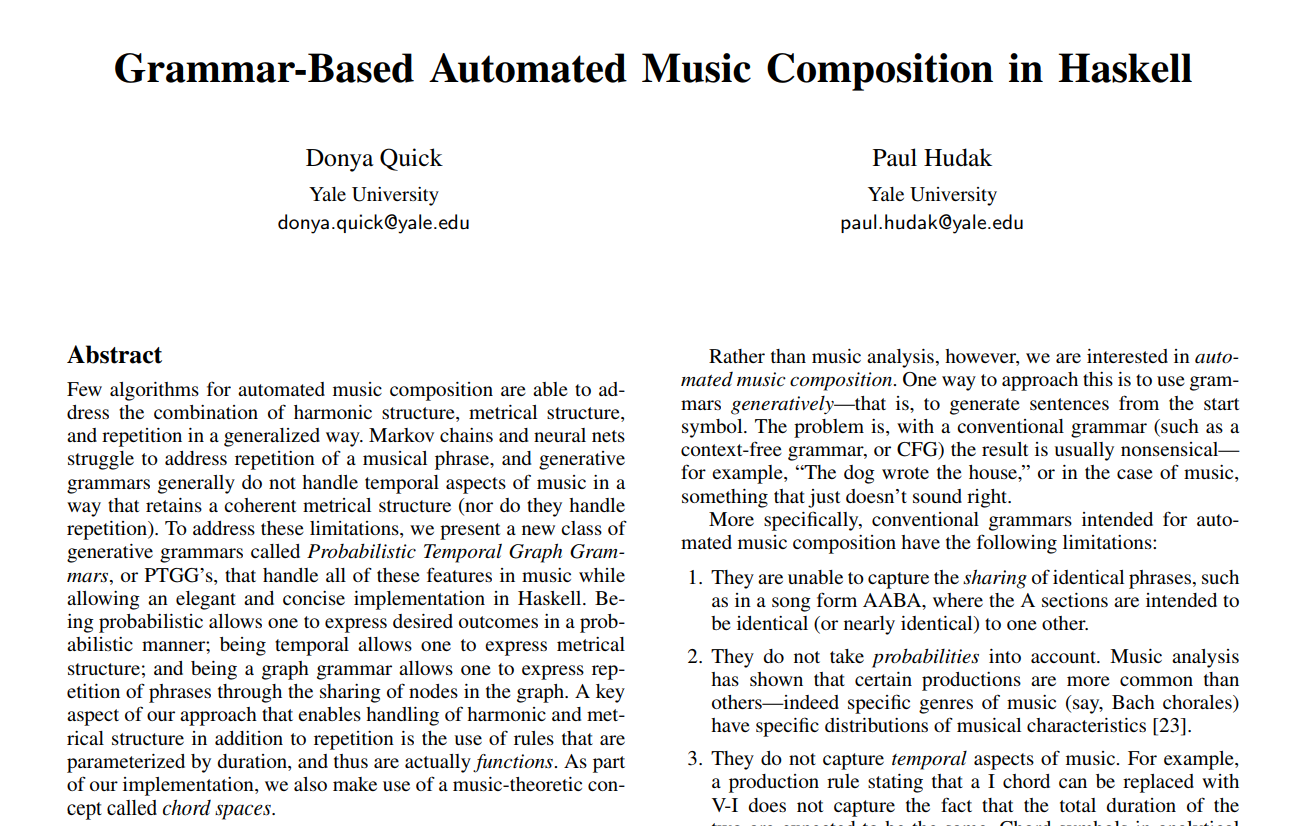
\includegraphics[keepaspectratio=true,height=.5\paperheight]{source-ptgg.png}
\end{frame}

\begin{frame}{Probabilistic Temporal Graph Grammars}
\begin{itemize}
\item \textbf{Probabilistic:} Rules are assigned prob. weights
\item \textbf{Temporal:} Rules are time-parametric
\item \textbf{Graph:} \ensuremath{\HSCon{Let}} construct allows sharing/repetition
\end{itemize}
\end{frame}

\begin{frame}{Euterpea}
\begin{itemize}
\item Euterpea will be our music development vehicle
\item Define some extra things that are not in the library
  \begin{enumerate}
  \item intervals, chords, scales
  \item transposition on several music elements
  \item random actions in \ensuremath{\HSCon{MonadRandom}}
  \end{enumerate}
\end{itemize}
\end{frame}

\begin{frame}{Intervals, Chords/Scales}
\begin{hs}\begin{hscode}\SaveRestoreHook
\column{B}{@{}>{\hspre}l<{\hspost}@{}}%
\column{3}{@{}>{\hspre}l<{\hspost}@{}}%
\column{9}{@{}>{\hspre}l<{\hspost}@{}}%
\column{14}{@{}>{\hspre}l<{\hspost}@{}}%
\column{17}{@{}>{\hspre}c<{\hspost}@{}}%
\column{17E}{@{}l@{}}%
\column{20}{@{}>{\hspre}l<{\hspost}@{}}%
\column{21}{@{}>{\hspre}l<{\hspost}@{}}%
\column{28}{@{}>{\hspre}l<{\hspost}@{}}%
\column{34}{@{}>{\hspre}l<{\hspost}@{}}%
\column{35}{@{}>{\hspre}l<{\hspost}@{}}%
\column{41}{@{}>{\hspre}l<{\hspost}@{}}%
\column{49}{@{}>{\hspre}l<{\hspost}@{}}%
\column{57}{@{}>{\hspre}l<{\hspost}@{}}%
\column{E}{@{}>{\hspre}l<{\hspost}@{}}%
\>[B]{}\HSKeyword{data}\;\HSCon{Interval}{}\<[E]%
\\
\>[B]{}\hsindent{3}{}\<[3]%
\>[3]{}\HSSym{\mathrel{=}}{}\<[9]%
\>[9]{}\HSCon{P1}{}\<[14]%
\>[14]{}\HSSym{\mathbin{\mid}}\HSCon{Mi2}{}\<[21]%
\>[21]{}\HSSym{\mathbin{\mid}}\HSCon{M2}{}\<[28]%
\>[28]{}\HSSym{\mathbin{\mid}}\HSCon{Mi3}{}\<[35]%
\>[35]{}\HSSym{\mathbin{\mid}}\HSCon{M3}{}\<[41]%
\>[41]{}\HSSym{\mathbin{\mid}}\HSCon{P4}{}\<[49]%
\>[49]{}\HSSym{\mathbin{\mid}}\HSCon{A4}{}\<[57]%
\>[57]{}\HSSym{\mathbin{\mid}}\HSCon{P5}{}\<[E]%
\\
\>[B]{}\hsindent{3}{}\<[3]%
\>[3]{}\;\HSSym{\mathbin{\mid}}{}\<[9]%
\>[9]{}\HSCon{Mi6}{}\<[14]%
\>[14]{}\HSSym{\mathbin{\mid}}\HSCon{M6}{}\<[21]%
\>[21]{}\HSSym{\mathbin{\mid}}\HSCon{Mi7}{}\<[28]%
\>[28]{}\HSSym{\mathbin{\mid}}\HSCon{M7}{}\<[35]%
\>[35]{}\HSSym{\mathbin{\mid}}\HSCon{P8}{}\<[41]%
\>[41]{}\HSSym{\mathbin{\mid}}\HSCon{Mi9}{}\<[49]%
\>[49]{}\HSSym{\mathbin{\mid}}\HSSym{\dots}{}\<[57]%
\>[57]{}\HSSym{\mathbin{\mid}}\HSCon{P15}{}\<[E]%
\\
\>[B]{}\hsindent{3}{}\<[3]%
\>[3]{}\HSKeyword{deriving}\;\HSSpecial{(}\HSCon{Eq}\HSSpecial{,}\HSCon{Enum}\HSSpecial{)}{}\<[E]%
\\
\>[B]{}\vspace{5pt}{}\<[E]%
\\
\>[B]{}\HSKeyword{type}\;\HSCon{ChordType}{}\<[17]%
\>[17]{}\HSSym{\mathrel{=}}{}\<[17E]%
\>[20]{}\HSSpecial{[\mskip1.5mu }\HSCon{Interval}\HSSpecial{\mskip1.5mu]}{}\<[34]%
\>[34]{}\HSComment{ -\! - $\equiv$ ScaleType}{}\<[E]%
\\
\>[B]{}\HSKeyword{type}\;\HSCon{SemiChord}{}\<[17]%
\>[17]{}\HSSym{\mathrel{=}}{}\<[17E]%
\>[20]{}\HSSpecial{[\mskip1.5mu }\HSCon{PitchClass}\HSSpecial{\mskip1.5mu]}{}\<[34]%
\>[34]{}\HSComment{ -\! - $\equiv$ SemiScale}{}\<[E]%
\\
\>[B]{}\HSKeyword{type}\;\HSCon{Chord}{}\<[17]%
\>[17]{}\HSSym{\mathrel{=}}{}\<[17E]%
\>[20]{}\HSSpecial{[\mskip1.5mu }\HSCon{Pitch}\HSSpecial{\mskip1.5mu]}{}\<[34]%
\>[34]{}\HSComment{ -\! - $\equiv$ Scale}{}\<[E]%
\\[\blanklineskip]%
\>[B]{}\HSSpecial{(}\HSSym{\ \mathbin{\Vdash}}\HSSpecial{)}\HSSym{::}\HSCon{PitchClass}\HSSym{\to} \HSCon{ChordType}\HSSym{\to} \HSCon{SemiChord}{}\<[E]%
\\
\>[B]{}\HSSpecial{(}\HSSym{\ \mathbin{\Vdash}}\HSSpecial{)}\HSSym{\mathrel{=}}\HSSym{\dots}{}\<[E]%
\ColumnHook
\end{hscode}\resethooks
\end{hs}
\end{frame}

\begin{frame}{A fairly extensive set of scales/chords}
\begin{hs}\begin{hscode}\SaveRestoreHook
\column{B}{@{}>{\hspre}l<{\hspost}@{}}%
\column{7}{@{}>{\hspre}c<{\hspost}@{}}%
\column{7E}{@{}l@{}}%
\column{9}{@{}>{\hspre}l<{\hspost}@{}}%
\column{10}{@{}>{\hspre}l<{\hspost}@{}}%
\column{12}{@{}>{\hspre}l<{\hspost}@{}}%
\column{E}{@{}>{\hspre}l<{\hspost}@{}}%
\>[B]{}\HSComment{ -\! - Chord types.}{}\<[E]%
\\
\>[B]{}\HSVar{maj}{}\<[7]%
\>[7]{}\HSSym{\mathrel{=}}{}\<[7E]%
\>[10]{}\HSSpecial{[\mskip1.5mu }\HSCon{P1}\HSSpecial{,}\HSCon{M3}\HSSpecial{,}\HSCon{P5}\HSSpecial{\mskip1.5mu]}{}\<[E]%
\\
\>[B]{}\HSVar{m7b5}{}\<[7]%
\>[7]{}\HSSym{\mathrel{=}}{}\<[7E]%
\>[10]{}\HSSpecial{[\mskip1.5mu }\HSCon{P1}\HSSpecial{,}\HSCon{Mi3}\HSSpecial{,}\HSCon{A4}\HSSpecial{,}\HSCon{Mi7}\HSSpecial{\mskip1.5mu]}{}\<[E]%
\\
\>[B]{}\HSSym{\vdots}{}\<[E]%
\\
\>[B]{}\HSVar{allChords}\HSSym{\mathrel{=}}\HSSpecial{[\mskip1.5mu }\HSVar{maj}\HSSpecial{,}\HSSym{\dots}\HSSpecial{\mskip1.5mu]}\HSSym{::}\HSSpecial{[\mskip1.5mu }\HSCon{ChordType}\HSSpecial{\mskip1.5mu]}{}\<[E]%
\\
\>[B]{}\vspace{5pt}{}\<[E]%
\\
\>[B]{}\HSComment{ -\! - Scale types.}{}\<[E]%
\\
\>[B]{}\HSVar{ionian}{}\<[9]%
\>[9]{}\HSSym{\mathrel{=}}\HSSpecial{[\mskip1.5mu }\HSCon{P1}\HSSpecial{,}\HSCon{M2}\HSSpecial{,}\HSCon{M3}\HSSpecial{,}\HSCon{P4}\HSSpecial{,}\HSCon{P5}\HSSpecial{,}\HSCon{M6}\HSSpecial{,}\HSCon{M7}\HSSpecial{\mskip1.5mu]}{}\<[E]%
\\
\>[B]{}\HSVar{major}{}\<[9]%
\>[9]{}\HSSym{\mathrel{=}}\HSVar{ionian}{}\<[E]%
\\
\>[B]{}\HSVar{lydian}{}\<[9]%
\>[9]{}\HSSym{\mathrel{=}}{}\<[12]%
\>[12]{}\HSVar{mode}\;\HSNumeral{4}\;\HSVar{ionian}{}\<[E]%
\\
\>[B]{}\HSSym{\vdots}{}\<[E]%
\\
\>[B]{}\HSVar{allScales}\HSSym{\mathrel{=}}\HSSpecial{[\mskip1.5mu }\HSVar{ionian}\HSSpecial{,}\HSSym{\dots}\HSSpecial{\mskip1.5mu]}\HSSym{::}\HSSpecial{[\mskip1.5mu }\HSCon{ScaleType}\HSSpecial{\mskip1.5mu]}{}\<[E]%
\ColumnHook
\end{hscode}\resethooks
\end{hs}
\end{frame}

\begin{frame}{Transposition}
\begin{hs}\begin{hscode}\SaveRestoreHook
\column{B}{@{}>{\hspre}l<{\hspost}@{}}%
\column{3}{@{}>{\hspre}l<{\hspost}@{}}%
\column{E}{@{}>{\hspre}l<{\hspost}@{}}%
\>[B]{}\HSKeyword{class}\;\HSCon{Transposable}\;\HSVar{a}\;\HSKeyword{where}{}\<[E]%
\\
\>[B]{}\hsindent{3}{}\<[3]%
\>[3]{}\HSSpecial{(}\HSSym{\mathbin{\uparrow}}\HSSpecial{)}\HSSpecial{,}\HSSpecial{(}\HSSym{\mathbin{\downarrow}}\HSSpecial{)}\HSSym{::}\HSVar{a}\HSSym{\to} \HSCon{Interval}\HSSym{\to} \HSVar{a}{}\<[E]%
\\
\>[B]{}\vspace{5pt}{}\<[E]%
\\
\>[B]{}\HSKeyword{instance}\;\HSCon{Transposable}\;\HSCon{PitchClass}\;\HSKeyword{where}\;\HSSym{\dots}{}\<[E]%
\\
\>[B]{}\HSKeyword{instance}\;\HSCon{Transposable}\;\HSCon{Chord}\;\HSKeyword{where}\;\HSSym{\dots}{}\<[E]%
\ColumnHook
\end{hscode}\resethooks
\end{hs}
\end{frame}

\begin{frame}{Random actions}
\begin{hs}\begin{hscode}\SaveRestoreHook
\column{B}{@{}>{\hspre}l<{\hspost}@{}}%
\column{3}{@{}>{\hspre}l<{\hspost}@{}}%
\column{E}{@{}>{\hspre}l<{\hspost}@{}}%
\>[B]{}\HSVar{equally}\HSSym{::}\HSSpecial{[\mskip1.5mu }\HSVar{a}\HSSpecial{\mskip1.5mu]}\HSSym{\to} \HSSpecial{[\mskip1.5mu }\HSSpecial{(}\HSCon{Double}\HSSpecial{,}\HSVar{a}\HSSpecial{)}\HSSpecial{\mskip1.5mu]}{}\<[E]%
\\
\>[B]{}\HSVar{equally}\HSSym{\mathrel{=}}\HSVar{zip}\;\HSSpecial{(}\HSVar{repeat}\;\HSNumeral{1.0}\HSSpecial{)}{}\<[E]%
\\
\>[B]{}\vspace{5pt}{}\<[E]%
\\
\>[B]{}\HSVar{choose}\HSSym{::}\HSCon{MonadRandom}\;\HSVar{m}\HSSym{\Rightarrow} \HSSpecial{[\mskip1.5mu }\HSSpecial{(}\HSCon{Double}\HSSpecial{,}\HSVar{a}\HSSpecial{)}\HSSpecial{\mskip1.5mu]}\HSSym{\to} \HSVar{m}\;\HSVar{a}{}\<[E]%
\\
\>[B]{}\HSVar{choose}\;\HSVar{xs}\HSSym{\mathrel{=}}\HSKeyword{do}{}\<[E]%
\\
\>[B]{}\hsindent{3}{}\<[3]%
\>[3]{}\HSVar{i}\HSSym{\leftarrow} \HSVar{getIndex}\HSSym{\mathbin{\langle\$\rangle}}\HSVar{getRandomR}\;\HSSpecial{(}\HSNumeral{0}\HSSpecial{,}\HSVar{sum}\;\HSSpecial{(}\HSVar{fst}\HSSym{\mathbin{\langle\$\rangle}}\HSVar{xs}\HSSpecial{)}\HSSpecial{)}{}\<[E]%
\\
\>[B]{}\hsindent{3}{}\<[3]%
\>[3]{}\HSVar{return}\;\HSSpecial{(}\HSVar{xs}\HSSym{\ \mathbin{!!}\ }\HSVar{i}\HSSpecial{)}{}\<[E]%
\\
\>[B]{}\vspace{5pt}{}\<[E]%
\\
\>[B]{}\HSVar{chooseBy}\HSSym{::}\HSCon{MonadRandom}\;\HSVar{m}\HSSym{\Rightarrow} \HSSpecial{(}\HSVar{a}\HSSym{\to} \HSCon{Double}\HSSpecial{)}\HSSym{\to} \HSSpecial{[\mskip1.5mu }\HSVar{a}\HSSpecial{\mskip1.5mu]}\HSSym{\to} \HSVar{m}\;\HSVar{a}{}\<[E]%
\\
\>[B]{}\HSVar{chooseBy}\HSSym{\mathrel{=}}\HSVar{choose}\HSSym{\mathbin{\circ}}\HSVar{fmap}\;\HSSpecial{(}\HSSym{\lambda} \HSVar{a}\HSSym{\to} \HSSpecial{(}\HSVar{f}\;\HSVar{a}\HSSpecial{,}\HSVar{a}\HSSpecial{)}\HSSpecial{)}{}\<[E]%
\ColumnHook
\end{hscode}\resethooks
\end{hs}
\end{frame}
\section{PTGG Extensions}

\begin{frame}{Grammars}
\begin{itemize}
\item A grammars consists of an initial symbol and several rewrite rules:
\begin{hs}\begin{hscode}\SaveRestoreHook
\column{B}{@{}>{\hspre}l<{\hspost}@{}}%
\column{3}{@{}>{\hspre}l<{\hspost}@{}}%
\column{E}{@{}>{\hspre}l<{\hspost}@{}}%
\>[B]{}\HSKeyword{data}\;\HSCon{Grammar}\;\HSVar{meta}\;\HSVar{a}{}\<[E]%
\\
\>[B]{}\hsindent{3}{}\<[3]%
\>[3]{}\HSSym{\mathrel{=}}\HSVar{a}\HSCon{\mathbin{\ |\!:}}\HSSpecial{[\mskip1.5mu }\HSCon{Rule}\;\HSVar{meta}\;\HSVar{a}\HSSpecial{\mskip1.5mu]}{}\<[E]%
\ColumnHook
\end{hscode}\resethooks
\end{hs}
\item A rule replaces an atomic symbol with a grammar term:
\begin{hs}\begin{hscode}\SaveRestoreHook
\column{B}{@{}>{\hspre}l<{\hspost}@{}}%
\column{3}{@{}>{\hspre}l<{\hspost}@{}}%
\column{E}{@{}>{\hspre}l<{\hspost}@{}}%
\>[B]{}\HSKeyword{data}\;\HSCon{Rule}\;\HSVar{meta}\;\HSVar{a}{}\<[E]%
\\
\>[B]{}\hsindent{3}{}\<[3]%
\>[3]{}\HSSym{\mathrel{=}}\HSSpecial{(}\HSVar{a}\HSSpecial{,}\HSCon{Double}\HSSpecial{,}\HSCon{Dur}\HSSym{\to} \HSCon{Bool}\HSSpecial{)}\HSCon{\mathbin{\rightarrowtail}}\HSSpecial{(}\HSCon{Dur}\HSSym{\to} \HSCon{Term}\;\HSVar{meta}\;\HSVar{a}\HSSpecial{)}{}\<[E]%
\ColumnHook
\end{hscode}\resethooks
\end{hs}
\end{itemize}
\end{frame}

\begin{frame}{Terms}
\begin{itemize}
\item Terms are (sequences of) atomic symbols, possibly wrapped with metadata or repeated with \ensuremath{\HSCon{Let}}:
\begin{hs}\begin{hscode}\SaveRestoreHook
\column{B}{@{}>{\hspre}l<{\hspost}@{}}%
\column{3}{@{}>{\hspre}c<{\hspost}@{}}%
\column{3E}{@{}l@{}}%
\column{6}{@{}>{\hspre}l<{\hspost}@{}}%
\column{E}{@{}>{\hspre}l<{\hspost}@{}}%
\>[B]{}\HSKeyword{data}\;\HSCon{Term}\;\HSVar{meta}\;\HSVar{a}{}\<[E]%
\\
\>[B]{}\hsindent{3}{}\<[3]%
\>[3]{}\HSSym{\mathrel{=}}{}\<[3E]%
\>[6]{}\HSVar{a}\HSSym{\mathbin{:}}\HSCon{Dur}{}\<[E]%
\\
\>[B]{}\hsindent{3}{}\<[3]%
\>[3]{}\HSSym{\mathbin{\mid}}{}\<[3E]%
\>[6]{}\HSCon{Term}\;\HSVar{meta}\;\HSVar{a}\HSCon{\mathbin{\ \otimes\ }}\HSCon{Term}\;\HSVar{meta}\;\HSVar{a}{}\<[E]%
\\
\>[B]{}\hsindent{3}{}\<[3]%
\>[3]{}\HSSym{\mathbin{\mid}}{}\<[3E]%
\>[6]{}\HSVar{meta}\HSCon{\mathbin{\vartriangleright}}\HSCon{Term}\;\HSVar{meta}\;\HSVar{a}{}\<[E]%
\\
\>[B]{}\hsindent{3}{}\<[3]%
\>[3]{}\HSSym{\mathbin{\mid}}{}\<[3E]%
\>[6]{}\HSCon{Let}\;\HSSpecial{(}\HSCon{Term}\;\HSVar{meta}\;\HSVar{a}\HSSpecial{)}\;\HSSpecial{(}\HSCon{Term}\;\HSVar{meta}\;\HSVar{a}\HSSym{\to} \HSCon{Term}\;\HSVar{meta}\;\HSVar{a}\HSSpecial{)}{}\<[E]%
\ColumnHook
\end{hscode}\resethooks
\end{hs}
\end{itemize}
\end{frame}

\begin{frame}{Expansion}
\begin{itemize}
\item The user has to provide a way to expand metadata:
\begin{hs}\begin{hscode}\SaveRestoreHook
\column{B}{@{}>{\hspre}l<{\hspost}@{}}%
\column{3}{@{}>{\hspre}l<{\hspost}@{}}%
\column{E}{@{}>{\hspre}l<{\hspost}@{}}%
\>[B]{}\HSKeyword{class}\;\HSCon{Expand}\;\HSVar{input}\;\HSVar{a}\;\HSVar{meta}\;\HSVar{b}\;\HSKeyword{where}{}\<[E]%
\\
\>[B]{}\hsindent{3}{}\<[3]%
\>[3]{}\HSVar{expand}\HSSym{::}\HSVar{input}\HSSym{\to} \HSCon{Term}\;\HSVar{meta}\;\HSVar{a}\HSSym{\to} \HSCon{IO}\;\HSSpecial{(}\HSCon{Term}\;\HSSpecial{(}\HSSpecial{)}\;\HSVar{b}\HSSpecial{)}{}\<[E]%
\ColumnHook
\end{hscode}\resethooks
\end{hs}
\end{itemize}
\end{frame}

\begin{frame}{Interpretation}
\begin{itemize}
\item The user has to provide a way to interpret abstract musical structures:
\begin{hs}\begin{hscode}\SaveRestoreHook
\column{B}{@{}>{\hspre}l<{\hspost}@{}}%
\column{3}{@{}>{\hspre}l<{\hspost}@{}}%
\column{E}{@{}>{\hspre}l<{\hspost}@{}}%
\>[B]{}\HSKeyword{class}\;\HSCon{ToMusic1}\;\HSVar{c}\HSSym{\Rightarrow} \HSCon{Interpret}\;\HSVar{input}\;\HSVar{b}\;\HSVar{c}\;\HSKeyword{where}{}\<[E]%
\\
\>[B]{}\hsindent{3}{}\<[3]%
\>[3]{}\HSVar{interpret}\HSSym{::}\HSVar{input}\HSSym{\to} \HSCon{Music}\;\HSVar{b}\HSSym{\to} \HSCon{IO}\;\HSSpecial{(}\HSCon{Music}\;\HSVar{c}\HSSpecial{)}{}\<[E]%
\ColumnHook
\end{hscode}\resethooks
\end{hs}
\end{itemize}
\end{frame}

\begin{frame}{User Constraints}
\begin{itemize}
\item All in all, the user makes sure the following constraints are satisfied:
\begin{hs}\begin{hscode}\SaveRestoreHook
\column{B}{@{}>{\hspre}l<{\hspost}@{}}%
\column{3}{@{}>{\hspre}l<{\hspost}@{}}%
\column{E}{@{}>{\hspre}l<{\hspost}@{}}%
\>[B]{}\HSKeyword{type}\;\HSCon{Grammarly}\;\HSVar{input}\;\HSVar{meta}\;\HSVar{a}\;\HSVar{b}\;\HSVar{c}\HSSym{\mathrel{=}}{}\<[E]%
\\
\>[B]{}\hsindent{3}{}\<[3]%
\>[3]{}\HSSpecial{(}\HSCon{Eq}\;\HSVar{a}\HSSpecial{,}\HSCon{Eq}\;\HSVar{meta}\HSSpecial{,}\HSCon{ToMusic1}\;\HSVar{c}{}\<[E]%
\\
\>[B]{}\hsindent{3}{}\<[3]%
\>[3]{}\HSSpecial{,}\HSCon{Expand}\;\HSVar{input}\;\HSVar{a}\;\HSVar{meta}\;\HSVar{b}{}\<[E]%
\\
\>[B]{}\hsindent{3}{}\<[3]%
\>[3]{}\HSSpecial{,}\HSCon{Interpret}\;\HSVar{input}\;\HSVar{b}\;\HSVar{c}\HSSpecial{)}{}\<[E]%
\ColumnHook
\end{hscode}\resethooks
\end{hs}
\end{itemize}
\end{frame}

\begin{frame}{Rewriting}
\begin{itemize}
\item Given a desired total duration, a well-formed grammar and the
required input for expansion and interpretation, rewrite up to fixpoint:
\begin{hs}\begin{hscode}\SaveRestoreHook
\column{B}{@{}>{\hspre}l<{\hspost}@{}}%
\column{3}{@{}>{\hspre}l<{\hspost}@{}}%
\column{13}{@{}>{\hspre}c<{\hspost}@{}}%
\column{13E}{@{}l@{}}%
\column{17}{@{}>{\hspre}l<{\hspost}@{}}%
\column{18}{@{}>{\hspre}l<{\hspost}@{}}%
\column{32}{@{}>{\hspre}l<{\hspost}@{}}%
\column{E}{@{}>{\hspre}l<{\hspost}@{}}%
\>[B]{}\HSVar{runGrammar}{}\<[13]%
\>[13]{}\HSSym{::}{}\<[13E]%
\>[18]{}\HSCon{Grammarly}\;\HSVar{input}\;\HSVar{meta}\;\HSVar{a}\;\HSVar{b}\;\HSVar{c}{}\<[E]%
\\
\>[13]{}\HSSym{\Rightarrow} {}\<[13E]%
\>[18]{}\HSCon{Grammar}\;\HSVar{meta}\;\HSVar{a}\HSSym{\to} \HSCon{Dur}\HSSym{\to} \HSVar{input}{}\<[E]%
\\
\>[13]{}\HSSym{\to} {}\<[13E]%
\>[18]{}\HSCon{IO}\;\HSSpecial{(}\HSCon{Music}\;\HSVar{b}\HSSpecial{,}{}\<[32]%
\>[32]{}\HSCon{Music1}\HSSpecial{)}{}\<[E]%
\\
\>[B]{}\HSVar{runGrammar}\;\HSSpecial{(}\HSVar{init}\HSCon{\mathbin{\ |\!:}}\HSVar{rs}\HSSpecial{)}\;\HSVar{t0}\;\HSVar{input}\HSSym{\mathrel{=}}\HSKeyword{do}{}\<[E]%
\\
\>[B]{}\hsindent{3}{}\<[3]%
\>[3]{}\HSVar{rewritten}{}\<[17]%
\>[17]{}\HSSym{\leftarrow} \HSVar{fixpointM}\;\HSVar{rewrite}\;\HSSpecial{(}\HSVar{init}\HSSym{\mathbin{:}}\HSVar{t0}\HSSpecial{)}{}\<[E]%
\\
\>[B]{}\hsindent{3}{}\<[3]%
\>[3]{}\HSVar{expanded}{}\<[17]%
\>[17]{}\HSSym{\leftarrow} \HSVar{expand}\;\HSVar{input}\;\HSSpecial{(}\HSVar{unlet}\;\HSVar{rewritten}\HSSpecial{)}{}\<[E]%
\\
\>[B]{}\hsindent{3}{}\<[3]%
\>[3]{}\HSKeyword{let}\;\HSVar{abstract}{}\<[17]%
\>[17]{}\HSSym{\mathrel{=}}\HSVar{toMusic}\;\HSVar{expanded}{}\<[E]%
\\
\>[B]{}\hsindent{3}{}\<[3]%
\>[3]{}\HSVar{concrete}{}\<[17]%
\>[17]{}\HSSym{\leftarrow} \HSVar{toMusic1}\HSSym{\mathbin{\langle\$\rangle}}\HSVar{interpret}\;\HSVar{input}\;\HSVar{abstract}{}\<[E]%
\\
\>[B]{}\hsindent{3}{}\<[3]%
\>[3]{}\HSVar{return}\;\HSSpecial{(}\HSVar{abstract}\HSSpecial{,}\HSVar{concrete}\HSSpecial{)}{}\<[E]%
\ColumnHook
\end{hscode}\resethooks
\end{hs}
\end{itemize}
\end{frame}

\section{Harmony}


\begin{frame}{Musicology Source: [Rohrmeier, 2011]}
\centering
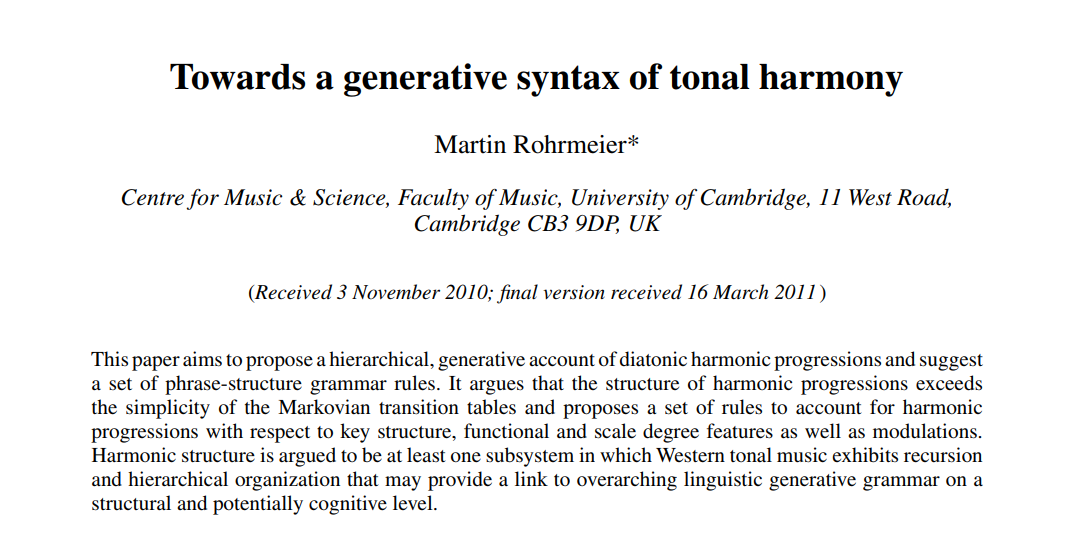
\includegraphics[keepaspectratio=true,height=.5\paperheight]{source-h.png}
\end{frame}

\begin{frame}{Grammar Symbols: Harmonic Degrees}
\begin{hs}\begin{hscode}\SaveRestoreHook
\column{B}{@{}>{\hspre}l<{\hspost}@{}}%
\column{3}{@{}>{\hspre}l<{\hspost}@{}}%
\column{8}{@{}>{\hspre}l<{\hspost}@{}}%
\column{11}{@{}>{\hspre}l<{\hspost}@{}}%
\column{17}{@{}>{\hspre}l<{\hspost}@{}}%
\column{24}{@{}>{\hspre}l<{\hspost}@{}}%
\column{30}{@{}>{\hspre}l<{\hspost}@{}}%
\column{35}{@{}>{\hspre}l<{\hspost}@{}}%
\column{41}{@{}>{\hspre}l<{\hspost}@{}}%
\column{48}{@{}>{\hspre}l<{\hspost}@{}}%
\column{E}{@{}>{\hspre}l<{\hspost}@{}}%
\>[B]{}\HSKeyword{data}\;\HSCon{Degree}{}\<[E]%
\\
\>[B]{}\hsindent{3}{}\<[3]%
\>[3]{}\HSSym{\mathrel{=}}{}\<[8]%
\>[8]{}\HSCon{I}{}\<[11]%
\>[11]{}\HSSym{\mathbin{\mid}}\HSCon{II}{}\<[17]%
\>[17]{}\HSSym{\mathbin{\mid}}\HSCon{III}{}\<[24]%
\>[24]{}\HSSym{\mathbin{\mid}}\HSCon{IV}{}\<[30]%
\>[30]{}\HSSym{\mathbin{\mid}}\HSCon{V}{}\<[35]%
\>[35]{}\HSSym{\mathbin{\mid}}\HSCon{VI}{}\<[41]%
\>[41]{}\HSSym{\mathbin{\mid}}\HSCon{VII}{}\<[48]%
\>[48]{}\HSComment{ -\! - terminals}{}\<[E]%
\\
\>[B]{}\hsindent{3}{}\<[3]%
\>[3]{}\HSSym{\ \mid}\;{}\<[8]%
\>[8]{}\HSCon{P}{}\<[11]%
\>[11]{}\HSSym{\mathbin{\mid}}\HSCon{TR}{}\<[17]%
\>[17]{}\HSSym{\mathbin{\mid}}\HSCon{DR}{}\<[24]%
\>[24]{}\HSSym{\mathbin{\mid}}\HSCon{SR}{}\<[30]%
\>[30]{}\HSSym{\mathbin{\mid}}\HSCon{T}{}\<[35]%
\>[35]{}\HSSym{\mathbin{\mid}}\HSCon{D}{}\<[41]%
\>[41]{}\HSSym{\mathbin{\mid}}\HSCon{S}{}\<[48]%
\>[48]{}\HSComment{ -\! - non-terminals}{}\<[E]%
\\
\>[B]{}\hsindent{3}{}\<[3]%
\>[3]{}\HSKeyword{deriving}\;\HSSpecial{(}\HSCon{Eq}\HSSpecial{,}\HSCon{Enum}\HSSpecial{)}{}\<[E]%
\ColumnHook
\end{hscode}\resethooks
\end{hs}
\end{frame}

\begin{frame}{Grammar for Western Tonal Harmony}
\savecolumns
\begin{hs}\begin{hscode}\SaveRestoreHook
\column{B}{@{}>{\hspre}l<{\hspost}@{}}%
\column{4}{@{}>{\hspre}c<{\hspost}@{}}%
\column{4E}{@{}l@{}}%
\column{7}{@{}>{\hspre}l<{\hspost}@{}}%
\column{12}{@{}>{\hspre}l<{\hspost}@{}}%
\column{24}{@{}>{\hspre}l<{\hspost}@{}}%
\column{32}{@{}>{\hspre}l<{\hspost}@{}}%
\column{38}{@{}>{\hspre}l<{\hspost}@{}}%
\column{47}{@{}>{\hspre}c<{\hspost}@{}}%
\column{47E}{@{}l@{}}%
\column{52}{@{}>{\hspre}l<{\hspost}@{}}%
\column{56}{@{}>{\hspre}l<{\hspost}@{}}%
\column{E}{@{}>{\hspre}l<{\hspost}@{}}%
\>[B]{}\HSVar{harmony}\HSSym{::}\HSCon{Grammar}\;\HSCon{Interval}\;\HSCon{Degree}{}\<[E]%
\\
\>[B]{}\HSVar{harmony}\HSSym{\mathrel{=}}\HSCon{P}\HSCon{\mathbin{\ |\!:}}{}\<[E]%
\\
\>[B]{}\hsindent{4}{}\<[4]%
\>[4]{}\HSSpecial{[\mskip1.5mu }{}\<[4E]%
\>[7]{}\HSComment{ -\! - Phrase level}{}\<[E]%
\\
\>[7]{}\HSSpecial{(}\HSCon{P}\HSSpecial{,}{}\<[12]%
\>[12]{}\HSNumeral{1}\HSSpecial{,}\HSVar{always}\HSSpecial{)}{}\<[24]%
\>[24]{}\HSCon{\mathbin{\rightarrowtail}}\HSSym{\lambda} \HSVar{t}\HSSym{\to} \HSVar{fillBars}\;\HSSpecial{(}\HSVar{t}\HSSpecial{,}\HSNumeral{4}\HSSym{*}\HSVar{wn}\HSSpecial{)}\;\HSCon{TR}{}\<[E]%
\\
\>[7]{}\HSComment{ -\! - Functional level: Expansion}{}\<[E]%
\\
\>[B]{}\hsindent{4}{}\<[4]%
\>[4]{}\HSSpecial{,}{}\<[4E]%
\>[7]{}\HSSpecial{(}\HSCon{TR}\HSSpecial{,}\HSNumeral{1}\HSSpecial{,}\HSSpecial{(}\HSSym{>}\HSVar{wn}\HSSpecial{)}\HSSpecial{)}{}\<[24]%
\>[24]{}\HSCon{\mathbin{\rightarrowtail}}\HSSym{\lambda} \HSVar{t}\HSSym{\to} \HSCon{TR}{}\<[38]%
\>[38]{}\HSSym{\mathbin{:}}\HSVar{t}\HSSym{\mathbin{\!/\!}}\HSNumeral{2}{}\<[47]%
\>[47]{}\HSCon{\mathbin{\ \otimes\ }}{}\<[47E]%
\>[52]{}\HSCon{DR}{}\<[56]%
\>[56]{}\HSSym{\mathbin{:}}\HSVar{t}\HSSym{\mathbin{\!/\!}}\HSNumeral{2}{}\<[E]%
\\
\>[B]{}\hsindent{4}{}\<[4]%
\>[4]{}\HSSpecial{,}{}\<[4E]%
\>[7]{}\HSSpecial{(}\HSCon{TR}\HSSpecial{,}\HSNumeral{1}\HSSpecial{,}\HSVar{always}\HSSpecial{)}{}\<[24]%
\>[24]{}\HSCon{\mathbin{\rightarrowtail}}\HSSym{\lambda} \HSVar{t}\HSSym{\to} \HSCon{DR}{}\<[38]%
\>[38]{}\HSSym{\mathbin{:}}\HSVar{t}\HSSym{\mathbin{\!/\!}}\HSNumeral{2}{}\<[47]%
\>[47]{}\HSCon{\mathbin{\ \otimes\ }}{}\<[47E]%
\>[52]{}\HSCon{T}{}\<[56]%
\>[56]{}\HSSym{\mathbin{:}}\HSVar{t}\HSSym{\mathbin{\!/\!}}\HSNumeral{2}{}\<[E]%
\\
\>[B]{}\hsindent{4}{}\<[4]%
\>[4]{}\HSSpecial{,}{}\<[4E]%
\>[7]{}\HSSpecial{(}\HSCon{DR}\HSSpecial{,}\HSNumeral{1}\HSSpecial{,}\HSVar{always}\HSSpecial{)}{}\<[24]%
\>[24]{}\HSCon{\mathbin{\rightarrowtail}}\HSSym{\lambda} \HSVar{t}\HSSym{\to} \HSCon{SR}{}\<[38]%
\>[38]{}\HSSym{\mathbin{:}}\HSVar{t}\HSSym{\mathbin{\!/\!}}\HSNumeral{2}{}\<[47]%
\>[47]{}\HSCon{\mathbin{\ \otimes\ }}{}\<[47E]%
\>[52]{}\HSCon{D}{}\<[56]%
\>[56]{}\HSSym{\mathbin{:}}\HSVar{t}\HSSym{\mathbin{\!/\!}}\HSNumeral{2}\;\HSSpecial{\mskip1.5mu]}\HSSym{\plus} {}\<[E]%
\\
\>[B]{}\hsindent{4}{}\<[4]%
\>[4]{}\HSSpecial{[\mskip1.5mu }{}\<[4E]%
\>[7]{}\HSSpecial{(}\HSVar{x}\HSSpecial{,}\HSNumeral{1}\HSSpecial{,}\HSSpecial{(}\HSSym{>}\HSVar{wn}\HSSpecial{)}\HSSpecial{)}\HSCon{\mathbin{\rightarrowtail}}\HSSym{\lambda} \HSVar{t}\HSSym{\to} \HSCon{Let}\;\HSSpecial{(}\HSVar{x}\HSSym{\mathbin{:}}\HSVar{t}\HSSym{\mathbin{\!/\!}}\HSNumeral{2}\HSSpecial{)}\;\HSSpecial{(}\HSSym{\lambda} \HSVar{y}\HSSym{\to} \HSVar{y}\HSCon{\mathbin{\ \otimes\ }}\HSVar{y}\HSSpecial{)}{}\<[E]%
\\
\>[B]{}\hsindent{4}{}\<[4]%
\>[4]{}\HSSym{\mathbin{\mid}}{}\<[4E]%
\>[7]{}\HSVar{x}\HSSym{\leftarrow} \HSSpecial{[\mskip1.5mu }\HSCon{TR}\HSSpecial{,}\HSCon{SR}\HSSpecial{,}\HSCon{DR}\HSSpecial{\mskip1.5mu]}\;\HSSpecial{\mskip1.5mu]}\HSSym{\plus} {}\<[E]%
\\
\>[B]{}\hsindent{4}{}\<[4]%
\>[4]{}\HSSpecial{[\mskip1.5mu }{}\<[4E]%
\>[7]{}\HSSpecial{(}\HSCon{TR}\HSSpecial{,}\HSNumeral{1}\HSSpecial{,}\HSVar{always}\HSSpecial{)}{}\<[24]%
\>[24]{}\HSCon{\mathbin{\rightarrowtail}}\HSSpecial{(}\HSCon{T}{}\<[32]%
\>[32]{}\HSSym{\ :}\HSSpecial{)}{}\<[E]%
\\
\>[B]{}\hsindent{4}{}\<[4]%
\>[4]{}\HSSpecial{,}{}\<[4E]%
\>[7]{}\HSSpecial{(}\HSCon{DR}\HSSpecial{,}\HSNumeral{1}\HSSpecial{,}\HSVar{always}\HSSpecial{)}{}\<[24]%
\>[24]{}\HSCon{\mathbin{\rightarrowtail}}\HSSpecial{(}\HSCon{D}{}\<[32]%
\>[32]{}\HSSym{\ :}\HSSpecial{)}{}\<[E]%
\\
\>[B]{}\hsindent{4}{}\<[4]%
\>[4]{}\HSSpecial{,}{}\<[4E]%
\>[7]{}\HSSpecial{(}\HSCon{SR}\HSSpecial{,}\HSNumeral{1}\HSSpecial{,}\HSVar{always}\HSSpecial{)}{}\<[24]%
\>[24]{}\HSCon{\mathbin{\rightarrowtail}}\HSSpecial{(}\HSCon{S}{}\<[32]%
\>[32]{}\HSSym{\ :}\HSSpecial{)}{}\<[E]%
\ColumnHook
\end{hscode}\resethooks
\end{hs}
\end{frame}

\begin{frame}{Grammar for Western Tonal Harmony}
\restorecolumns
\begin{hs}\begin{hscode}\SaveRestoreHook
\column{B}{@{}>{\hspre}l<{\hspost}@{}}%
\column{4}{@{}>{\hspre}c<{\hspost}@{}}%
\column{4E}{@{}l@{}}%
\column{7}{@{}>{\hspre}l<{\hspost}@{}}%
\column{24}{@{}>{\hspre}l<{\hspost}@{}}%
\column{33}{@{}>{\hspre}l<{\hspost}@{}}%
\column{38}{@{}>{\hspre}l<{\hspost}@{}}%
\column{44}{@{}>{\hspre}l<{\hspost}@{}}%
\column{E}{@{}>{\hspre}l<{\hspost}@{}}%
\>[7]{}\HSComment{ -\! - Functional level: Modulation}{}\<[E]%
\\
\>[4]{}\HSSpecial{,}{}\<[4E]%
\>[7]{}\HSSpecial{(}\HSCon{D}\HSSpecial{,}\HSNumeral{1}\HSSpecial{,}\HSSpecial{(}\HSSym{\geq} \HSVar{qn}\HSSpecial{)}\HSSpecial{)}{}\<[24]%
\>[24]{}\HSCon{\mathbin{\rightarrowtail}}\HSSym{\lambda} \HSVar{t}\HSSym{\to} \HSCon{P5}\HSCon{\mathbin{\vartriangleright}}\HSCon{D}{}\<[44]%
\>[44]{}\HSSym{\mathbin{:}}\HSVar{t}{}\<[E]%
\\
\>[4]{}\HSSpecial{,}{}\<[4E]%
\>[7]{}\HSSpecial{(}\HSCon{S}\HSSpecial{,}\HSNumeral{1}\HSSpecial{,}\HSSpecial{(}\HSSym{\geq} \HSVar{qn}\HSSpecial{)}\HSSpecial{)}{}\<[24]%
\>[24]{}\HSCon{\mathbin{\rightarrowtail}}\HSSym{\lambda} \HSVar{t}\HSSym{\to} \HSCon{P4}\HSCon{\mathbin{\vartriangleright}}\HSCon{S}{}\<[44]%
\>[44]{}\HSSym{\mathbin{:}}\HSVar{t}\;\HSSpecial{\mskip1.5mu]}\HSSym{\plus} {}\<[E]%
\\
\>[7]{}\HSComment{ -\! - Scale-degree level: Secondary dominants}{}\<[E]%
\\
\>[4]{}\HSSpecial{[\mskip1.5mu }{}\<[4E]%
\>[7]{}\HSSpecial{(}\HSVar{x}\HSSpecial{,}\HSNumeral{1}\HSSpecial{,}\HSSpecial{(}\HSSym{\geq} \HSVar{hn}\HSSpecial{)}\HSSpecial{)}\HSCon{\mathbin{\rightarrowtail}}\HSSym{\lambda} \HSVar{t}\HSSym{\to} \HSCon{Let}\;{}\<[38]%
\>[38]{}\HSSpecial{(}\HSVar{x}\HSSym{\mathbin{:}}\HSVar{t}\HSSym{\mathbin{\!/\!}}\HSNumeral{2}\HSSpecial{)}\;\HSSpecial{(}\HSSym{\lambda} \HSVar{y}\HSSym{\to} \HSSpecial{(}\HSCon{P5}\HSCon{\mathbin{\vartriangleright}}\HSVar{y}\HSSpecial{)}\HSCon{\mathbin{\ \otimes\ }}\HSVar{y}\HSSpecial{)}{}\<[E]%
\\
\>[4]{}\HSSym{\mathbin{\mid}}{}\<[4E]%
\>[7]{}\HSVar{x}\HSSym{\leftarrow} \HSSpecial{[\mskip1.5mu }\HSCon{T}\HSSpecial{,}\HSCon{D}\HSSpecial{,}\HSCon{S}\HSSpecial{\mskip1.5mu]}\;\HSSpecial{\mskip1.5mu]}\HSSym{\plus} {}\<[E]%
\\
\>[4]{}\HSSpecial{[\mskip1.5mu }{}\<[4E]%
\>[7]{}\HSComment{ -\! - Scale-degree level: Functional-Scale interface}{}\<[E]%
\\
\>[7]{}\HSSpecial{(}\HSCon{T}\HSSpecial{,}\HSNumeral{1}\HSSpecial{,}\HSSpecial{(}\HSSym{\geq} \HSVar{wn}\HSSpecial{)}\HSSpecial{)}{}\<[24]%
\>[24]{}\HSCon{\mathbin{\rightarrowtail}}\HSSym{\lambda} \HSVar{t}\HSSym{\to} \HSCon{I}\HSSym{\mathbin{:}}\HSVar{t}\HSSym{\mathbin{\!/\!}}\HSNumeral{2}\HSCon{\mathbin{\ \otimes\ }}\HSCon{IV}\HSSym{\mathbin{:}}\HSVar{t}\HSSym{\mathbin{\!/\!}}\HSNumeral{4}\HSCon{\mathbin{\ \otimes\ }}\HSCon{I}\HSSym{\mathbin{:}}\HSVar{t}\HSSym{\mathbin{\!/\!}}\HSNumeral{4}{}\<[E]%
\\
\>[4]{}\HSSpecial{,}{}\<[4E]%
\>[7]{}\HSSpecial{(}\HSCon{T}\HSSpecial{,}\HSNumeral{1}\HSSpecial{,}\HSVar{always}\HSSpecial{)}{}\<[24]%
\>[24]{}\HSCon{\mathbin{\rightarrowtail}}\HSSpecial{(}\HSCon{I}{}\<[33]%
\>[33]{}\HSSym{\ :}\HSSpecial{)}{}\<[E]%
\\
\>[4]{}\HSSpecial{,}{}\<[4E]%
\>[7]{}\HSSpecial{(}\HSCon{S}\HSSpecial{,}\HSNumeral{1}\HSSpecial{,}\HSVar{always}\HSSpecial{)}{}\<[24]%
\>[24]{}\HSCon{\mathbin{\rightarrowtail}}\HSSpecial{(}\HSCon{IV}{}\<[33]%
\>[33]{}\HSSym{\ :}\HSSpecial{)}{}\<[E]%
\\
\>[4]{}\HSSpecial{,}{}\<[4E]%
\>[7]{}\HSSpecial{(}\HSCon{D}\HSSpecial{,}\HSNumeral{1}\HSSpecial{,}\HSVar{always}\HSSpecial{)}{}\<[24]%
\>[24]{}\HSCon{\mathbin{\rightarrowtail}}\HSSpecial{(}\HSCon{V}{}\<[33]%
\>[33]{}\HSSym{\ :}\HSSpecial{)}{}\<[E]%
\\
\>[4]{}\HSSpecial{,}{}\<[4E]%
\>[7]{}\HSSpecial{(}\HSCon{D}\HSSpecial{,}\HSNumeral{1}\HSSpecial{,}\HSVar{always}\HSSpecial{)}{}\<[24]%
\>[24]{}\HSCon{\mathbin{\rightarrowtail}}\HSSpecial{(}\HSCon{VI}{}\<[33]%
\>[33]{}\HSSym{\ :}\HSSpecial{)}\;\HSSpecial{\mskip1.5mu]}{}\<[E]%
\ColumnHook
\end{hscode}\resethooks
\end{hs}
\end{frame}

\begin{frame}{Expansion: Key Modulation}
\begin{hs}\begin{hscode}\SaveRestoreHook
\column{B}{@{}>{\hspre}l<{\hspost}@{}}%
\column{3}{@{}>{\hspre}l<{\hspost}@{}}%
\column{6}{@{}>{\hspre}l<{\hspost}@{}}%
\column{11}{@{}>{\hspre}c<{\hspost}@{}}%
\column{11E}{@{}l@{}}%
\column{15}{@{}>{\hspre}l<{\hspost}@{}}%
\column{17}{@{}>{\hspre}c<{\hspost}@{}}%
\column{17E}{@{}l@{}}%
\column{21}{@{}>{\hspre}l<{\hspost}@{}}%
\column{31}{@{}>{\hspre}l<{\hspost}@{}}%
\column{32}{@{}>{\hspre}l<{\hspost}@{}}%
\column{E}{@{}>{\hspre}l<{\hspost}@{}}%
\>[B]{}\HSKeyword{data}\;\HSCon{HarmonyConfig}\HSSym{\mathrel{=}}\HSCon{HarmonyConfig}{}\<[E]%
\\
\>[B]{}\hsindent{3}{}\<[3]%
\>[3]{}\HSSpecial{\{\mskip1.5mu }{}\<[6]%
\>[6]{}\HSVar{basePc}{}\<[17]%
\>[17]{}\HSSym{::}{}\<[17E]%
\>[21]{}\HSCon{PitchClass}{}\<[E]%
\\
\>[B]{}\hsindent{3}{}\<[3]%
\>[3]{}\HSSpecial{,}{}\<[6]%
\>[6]{}\HSVar{baseScale}{}\<[17]%
\>[17]{}\HSSym{::}{}\<[17E]%
\>[21]{}\HSCon{ScaleType}{}\<[E]%
\\
\>[B]{}\hsindent{3}{}\<[3]%
\>[3]{}\HSSpecial{,}{}\<[6]%
\>[6]{}\HSVar{chords}{}\<[17]%
\>[17]{}\HSSym{::}{}\<[17E]%
\>[21]{}\HSSpecial{[\mskip1.5mu }\HSSpecial{(}\HSCon{Double}\HSSpecial{,}\HSCon{ChordType}\HSSpecial{)}\HSSpecial{\mskip1.5mu]}\;\HSSpecial{\mskip1.5mu\}}{}\<[E]%
\\
\>[B]{}\vspace{5pt}{}\<[E]%
\\
\>[B]{}\HSKeyword{instance}\;\HSCon{Expand}\;\HSCon{HarmonyConfig}\;{}\<[32]%
\>[32]{}\HSCon{Degree}\;\HSCon{Interval}\;\HSCon{SemiChord}\;\HSKeyword{where}{}\<[E]%
\\
\>[B]{}\hsindent{3}{}\<[3]%
\>[3]{}\HSVar{expand}{}\<[11]%
\>[11]{}\HSSym{::}{}\<[11E]%
\>[15]{}\HSCon{HarmonyConfig}\HSSym{\to} \HSCon{Term}\;\HSCon{Interval}\;\HSCon{Degree}{}\<[E]%
\\
\>[11]{}\HSSym{\to} {}\<[11E]%
\>[15]{}\HSCon{IO}\;\HSSpecial{(}\HSCon{Term}\;\HSSpecial{(}\HSSpecial{)}\;\HSCon{SemiChord}\HSSpecial{)}{}\<[E]%
\\
\>[B]{}\hsindent{3}{}\<[3]%
\>[3]{}\HSVar{expand}\;\HSVar{cfg}\;{}\<[15]%
\>[15]{}\HSSpecial{(}\HSVar{i}\HSCon{\mathbin{\vartriangleright}}\HSVar{e}\HSSpecial{)}{}\<[31]%
\>[31]{}\HSSym{\mathrel{=}}\HSVar{expand}\;\HSSpecial{(}\HSVar{cfg}\;\HSSpecial{\{\mskip1.5mu }\HSVar{basePc}\HSSym{\mathrel{=}}\HSVar{basePc}\;\HSVar{cfg}\HSSym{\mathbin{\uparrow}}\HSVar{i}\HSSpecial{\mskip1.5mu\}}\HSSpecial{)}\;\HSVar{e}{}\<[E]%
\\
\>[B]{}\hsindent{3}{}\<[3]%
\>[3]{}\HSSym{\dots}{}\<[E]%
\\
\>[B]{}\hsindent{3}{}\<[3]%
\>[3]{}\HSVar{expand}\;\HSVar{cfg}\;{}\<[15]%
\>[15]{}\HSSpecial{(}\HSVar{degree}\HSSym{\mathbin{:}}\HSVar{t}\HSSpecial{)}{}\<[31]%
\>[31]{}\HSSym{\mathrel{=}}\HSSpecial{(}\HSSym{\mathbin{:}}\HSVar{t}\HSSpecial{)}\HSSym{\mathbin{\langle\$\rangle}}\HSVar{choose}\;\HSSpecial{(}\HSVar{filterChords}\;\HSVar{cfg}\;\HSVar{degree}\HSSpecial{)}{}\<[E]%
\ColumnHook
\end{hscode}\resethooks
\end{hs}
\end{frame}

\begin{frame}{Interpretation: From Abstract to Semi Chords}
\begin{hs}\begin{hscode}\SaveRestoreHook
\column{B}{@{}>{\hspre}l<{\hspost}@{}}%
\column{3}{@{}>{\hspre}l<{\hspost}@{}}%
\column{5}{@{}>{\hspre}l<{\hspost}@{}}%
\column{7}{@{}>{\hspre}l<{\hspost}@{}}%
\column{E}{@{}>{\hspre}l<{\hspost}@{}}%
\>[B]{}\HSKeyword{instance}\;\HSCon{Interpret}\;\HSCon{HarmonyConfig}\;\HSCon{SemiChord}\;\HSCon{Chord}\;\HSKeyword{where}{}\<[E]%
\\
\>[B]{}\hsindent{3}{}\<[3]%
\>[3]{}\HSVar{interpret}\HSSym{::}\HSCon{HarmonyConfig}\HSSym{\to} \HSCon{Music}\;\HSCon{SemiChord}\HSSym{\to} \HSCon{IO}\;\HSSpecial{(}\HSCon{Music}\;\HSCon{Chord}\HSSpecial{)}{}\<[E]%
\\
\>[B]{}\hsindent{3}{}\<[3]%
\>[3]{}\HSVar{interpret}\;\HSVar{cfg}\HSSym{\mathrel{=}}\HSVar{fold1}\;\HSVar{f}{}\<[E]%
\\
\>[3]{}\hsindent{2}{}\<[5]%
\>[5]{}\HSKeyword{where}\;\HSVar{f}\;\HSVar{m}\;\HSSpecial{(}\HSVar{sc}\HSSpecial{,}\HSVar{d}\HSSpecial{)}\HSSym{\mathrel{=}}\HSKeyword{do}{}\<[E]%
\\
\>[5]{}\hsindent{2}{}\<[7]%
\>[7]{}\HSVar{ch}\HSSym{\leftarrow} \HSVar{chooseBy}\;\HSSpecial{(}\HSVar{chordDistance}\;\HSVar{m}\HSSpecial{)}\;\HSSpecial{(}\HSVar{inversions}\;\HSVar{sc}\HSSpecial{)}{}\<[E]%
\\
\>[5]{}\hsindent{2}{}\<[7]%
\>[7]{}\HSVar{return}\;\HSSpecial{(}\HSVar{m}\HSCon{\mathbin{\ \otimes\ }}\HSVar{ch}\HSSpecial{)}{}\<[E]%
\ColumnHook
\end{hscode}\resethooks
\end{hs}
\end{frame}

\begin{frame}{Rewrite Example}
\centering

\ensuremath{\HSCon{P}\HSSym{\mathbin{:}}\HSNumeral{8}\HSSym{*}\HSVar{wn}}

\pause

\ensuremath{\HSSym{\mathbin{\downarrow}}}

\ensuremath{\HSCon{TR}\HSSym{\mathbin{:}}\HSNumeral{4}\HSSym{*}\HSVar{wn}\HSCon{\mathbin{\ \otimes\ }}\HSCon{TR}\HSSym{\mathbin{:}}\HSNumeral{4}\HSSym{*}\HSVar{wn}}

\pause

\ensuremath{\HSSym{\mathbin{\downarrow}}}

\ensuremath{\HSCon{TR}\HSSym{\mathbin{:}}\HSNumeral{2}\HSSym{*}\HSVar{wn}\HSCon{\mathbin{\ \otimes\ }}\HSCon{DR}\HSSym{\mathbin{:}}\HSNumeral{2}\HSSym{*}\HSVar{wn}\HSCon{\mathbin{\ \otimes\ }}\HSCon{TR}\HSSym{\mathbin{:}}\HSNumeral{2}\HSSym{*}\HSVar{wn}}

\pause

\ensuremath{\HSSym{\vdots}}

\ensuremath{\HSSym{\mathbin{\downarrow}}}

\ensuremath{\HSCon{I}\HSSym{\mathbin{:}}\HSVar{wn}\HSCon{\mathbin{\ \otimes\ }}\HSCon{IV}\HSSym{\mathbin{:}}\HSVar{hn}\;\HSCon{I}\HSSym{\mathbin{:}}\HSVar{hn}\HSCon{\mathbin{\ \otimes\ }}\HSSpecial{(}\HSCon{P5}\HSCon{\mathbin{\vartriangleright}}\HSCon{VI}\HSSym{\mathbin{:}}\HSVar{wn}\HSSpecial{)}\HSCon{\mathbin{\ \otimes\ }}\HSCon{V}\HSSym{\mathbin{:}}\HSVar{wn}\HSCon{\mathbin{\ \otimes\ }}\HSCon{I}\HSSym{\mathbin{:}}\HSNumeral{2}\HSSym{*}\HSVar{wn}}
\end{frame}
\section{Melody}

\begin{frame}{Musicology Source: [Keller, 2007]}
\centering
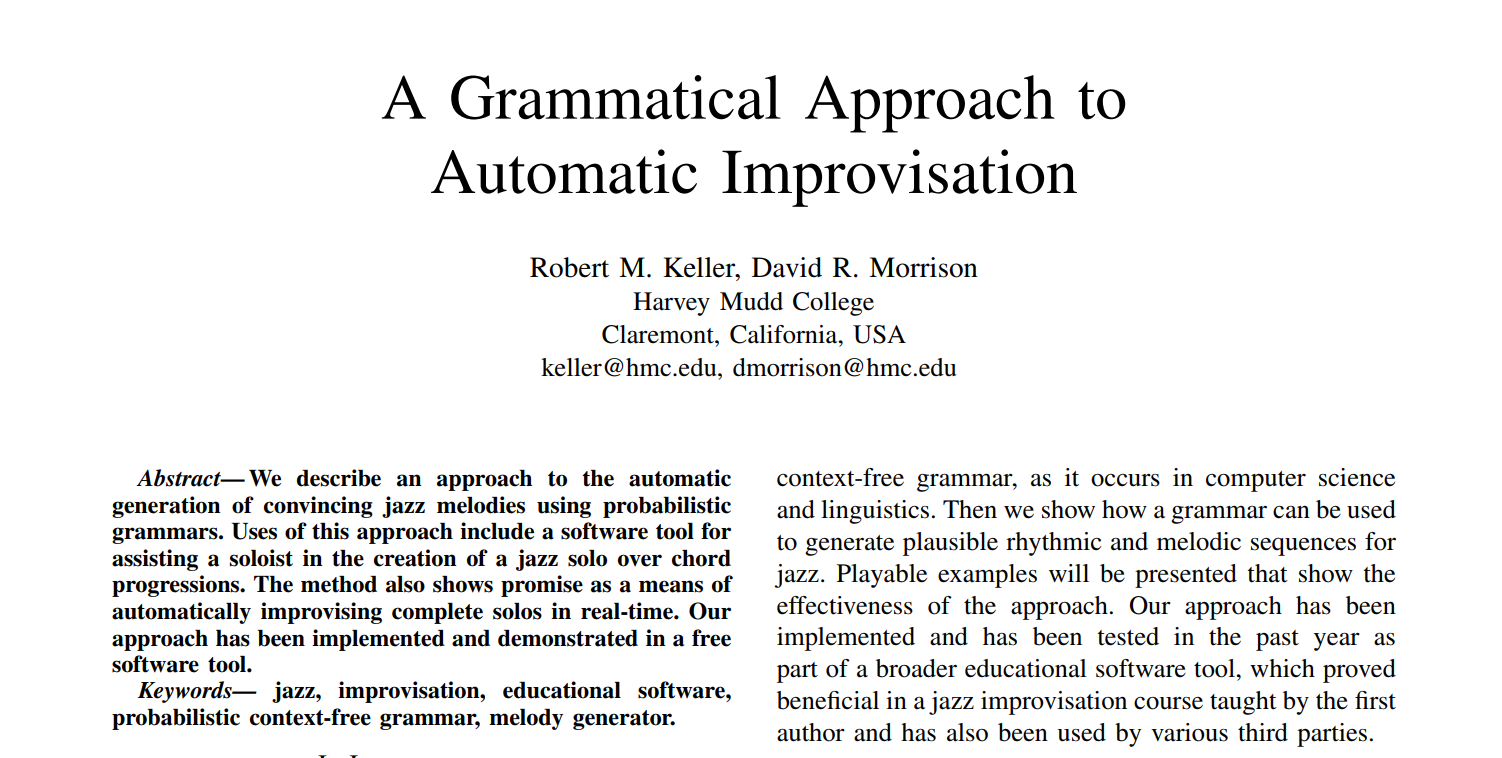
\includegraphics[keepaspectratio=true,height=.5\paperheight]{source-m.png}
\end{frame}

\begin{frame}{Grammar Symbols: Tones}
\begin{hs}\begin{hscode}\SaveRestoreHook
\column{B}{@{}>{\hspre}l<{\hspost}@{}}%
\column{3}{@{}>{\hspre}l<{\hspost}@{}}%
\column{6}{@{}>{\hspre}l<{\hspost}@{}}%
\column{10}{@{}>{\hspre}l<{\hspost}@{}}%
\column{16}{@{}>{\hspre}l<{\hspost}@{}}%
\column{21}{@{}>{\hspre}l<{\hspost}@{}}%
\column{36}{@{}>{\hspre}l<{\hspost}@{}}%
\column{E}{@{}>{\hspre}l<{\hspost}@{}}%
\>[B]{}\HSKeyword{data}\;\HSCon{M}{}\<[E]%
\\
\>[B]{}\hsindent{3}{}\<[3]%
\>[3]{}\HSSym{\mathrel{=}}{}\<[6]%
\>[6]{}\HSCon{HT}{}\<[10]%
\>[10]{}\HSSym{\mathbin{\mid}}\HSCon{CT}{}\<[16]%
\>[16]{}\HSSym{\mathbin{\mid}}\HSCon{L}{}\<[21]%
\>[21]{}\HSSym{\mathbin{\mid}}\HSCon{AT}\HSSym{\mathbin{\mid}}\HSCon{ST}\HSSym{\mathbin{\mid}}\HSCon{R}{}\<[36]%
\>[36]{}\HSComment{ -\! - terminals}{}\<[E]%
\\
\>[B]{}\hsindent{3}{}\<[3]%
\>[3]{}\HSSym{\mathbin{\mid}}{}\<[6]%
\>[6]{}\HSCon{P}{}\<[10]%
\>[10]{}\HSSym{\mathbin{\mid}}\HSCon{Q}{}\<[16]%
\>[16]{}\HSSym{\mathbin{\mid}}\HSCon{V}{}\<[21]%
\>[21]{}\HSSym{\mathbin{\mid}}\HSCon{N}{}\<[36]%
\>[36]{}\HSComment{ -\! - non-terminals}{}\<[E]%
\\
\>[B]{}\hsindent{3}{}\<[3]%
\>[3]{}\HSKeyword{deriving}\;\HSCon{Eq}{}\<[E]%
\\
\>[B]{}\vspace{5pt}{}\<[E]%
\\
\>[B]{}\HSSpecial{(}\HSCon{\mathbin{\rightarrowtriangle}}\HSSpecial{)}\HSSym{::}\HSSpecial{(}\HSVar{a}\HSSpecial{,}\HSCon{Double}\HSSpecial{,}\HSCon{Dur}\HSSym{\to} \HSCon{Bool}\HSSpecial{)}\HSSym{\to} \HSCon{Term}\;\HSVar{meta}\;\HSVar{a}\HSSym{\to} \HSCon{Rule}\;\HSVar{meta}\;\HSVar{a}{}\<[E]%
\\
\>[B]{}\HSVar{a}\HSCon{\mathbin{\rightarrowtriangle}}\HSVar{b}\HSSym{\mathrel{=}}\HSVar{a}\HSCon{\mathbin{\rightarrowtail}}\HSVar{const}\;\HSVar{b}{}\<[E]%
\ColumnHook
\end{hscode}\resethooks
\end{hs}
\end{frame}

\begin{frame}{Grammar for Melodic Jazz Improvisation}
\savecolumns
\begin{hs}\begin{hscode}\SaveRestoreHook
\column{B}{@{}>{\hspre}l<{\hspost}@{}}%
\column{3}{@{}>{\hspre}c<{\hspost}@{}}%
\column{3E}{@{}l@{}}%
\column{6}{@{}>{\hspre}l<{\hspost}@{}}%
\column{11}{@{}>{\hspre}l<{\hspost}@{}}%
\column{15}{@{}>{\hspre}l<{\hspost}@{}}%
\column{26}{@{}>{\hspre}c<{\hspost}@{}}%
\column{26E}{@{}l@{}}%
\column{31}{@{}>{\hspre}l<{\hspost}@{}}%
\column{47}{@{}>{\hspre}l<{\hspost}@{}}%
\column{E}{@{}>{\hspre}l<{\hspost}@{}}%
\>[B]{}\HSVar{melody}\HSSym{::}\HSCon{Grammar}\;\HSSpecial{(}\HSSpecial{)}\;\HSCon{M}{}\<[E]%
\\
\>[B]{}\HSVar{melody}\HSSym{\mathrel{=}}\HSCon{P}\HSCon{\mathbin{\ |\!:}}{}\<[E]%
\\
\>[B]{}\hsindent{3}{}\<[3]%
\>[3]{}\HSSpecial{[\mskip1.5mu }{}\<[3E]%
\>[6]{}\HSComment{ -\! - Rhythmic Structure: Expand P to Q}{}\<[E]%
\\
\>[6]{}\HSSpecial{(}\HSCon{P}\HSSpecial{,}{}\<[11]%
\>[11]{}\HSNumeral{1}\HSSpecial{,}{}\<[15]%
\>[15]{}\HSSpecial{(}\HSSym{\equiv} \HSVar{qn}\HSSpecial{)}\HSSpecial{)}{}\<[26]%
\>[26]{}\HSCon{\mathbin{\rightarrowtail}}{}\<[26E]%
\>[31]{}\HSSpecial{(}\HSCon{Q}\HSSym{\ :}\HSSpecial{)}{}\<[E]%
\\
\>[B]{}\hsindent{3}{}\<[3]%
\>[3]{}\HSSpecial{,}{}\<[3E]%
\>[6]{}\HSSpecial{(}\HSCon{P}\HSSpecial{,}{}\<[11]%
\>[11]{}\HSNumeral{1}\HSSpecial{,}{}\<[15]%
\>[15]{}\HSSpecial{(}\HSSym{\equiv} \HSVar{hn}\HSSpecial{)}\HSSpecial{)}{}\<[26]%
\>[26]{}\HSCon{\mathbin{\rightarrowtail}}{}\<[26E]%
\>[31]{}\HSSpecial{(}\HSCon{Q}\HSSym{\ :}\HSSpecial{)}{}\<[E]%
\\
\>[B]{}\hsindent{3}{}\<[3]%
\>[3]{}\HSSpecial{,}{}\<[3E]%
\>[6]{}\HSSpecial{(}\HSCon{P}\HSSpecial{,}{}\<[11]%
\>[11]{}\HSNumeral{1}\HSSpecial{,}{}\<[15]%
\>[15]{}\HSSpecial{(}\HSSym{\equiv} \HSVar{hn^{.}}\HSSpecial{)}\HSSpecial{)}{}\<[26]%
\>[26]{}\HSCon{\mathbin{\rightarrowtriangle}}{}\<[26E]%
\>[31]{}\HSCon{Q}\HSSym{\mathbin{:}}\HSVar{hn}\HSCon{\mathbin{\ \otimes\ }}\HSCon{Q}\HSSym{\mathbin{:}}\HSVar{qn}{}\<[E]%
\\
\>[B]{}\hsindent{3}{}\<[3]%
\>[3]{}\HSSpecial{,}{}\<[3E]%
\>[6]{}\HSSpecial{(}\HSCon{P}\HSSpecial{,}\HSNumeral{25}\HSSpecial{,}{}\<[15]%
\>[15]{}\HSSpecial{(}\HSSym{>}\HSVar{hn^{.}}\HSSpecial{)}\HSSpecial{)}{}\<[26]%
\>[26]{}\HSCon{\mathbin{\rightarrowtail}}{}\<[26E]%
\>[31]{}\HSSym{\lambda} \HSVar{t}\HSSym{\to} \HSCon{Q}\HSSym{\mathbin{:}}\HSVar{hn}{}\<[47]%
\>[47]{}\HSCon{\mathbin{\ \otimes\ }}\HSCon{P}\HSSym{\mathbin{:}}\HSSpecial{(}\HSVar{t}\HSSym{-}\HSVar{hn}\HSSpecial{)}{}\<[E]%
\\
\>[B]{}\hsindent{3}{}\<[3]%
\>[3]{}\HSSpecial{,}{}\<[3E]%
\>[6]{}\HSSpecial{(}\HSCon{P}\HSSpecial{,}\HSNumeral{75}\HSSpecial{,}{}\<[15]%
\>[15]{}\HSSpecial{(}\HSSym{>}\HSVar{wn}\HSSpecial{)}\HSSpecial{)}{}\<[26]%
\>[26]{}\HSCon{\mathbin{\rightarrowtail}}{}\<[26E]%
\>[31]{}\HSSym{\lambda} \HSVar{t}\HSSym{\to} \HSCon{Q}\HSSym{\mathbin{:}}\HSVar{wn}{}\<[47]%
\>[47]{}\HSCon{\mathbin{\ \otimes\ }}\HSCon{P}\HSSym{\mathbin{:}}\HSSpecial{(}\HSVar{t}\HSSym{-}\HSVar{wn}\HSSpecial{)}{}\<[E]%
\ColumnHook
\end{hscode}\resethooks
\end{hs}
\end{frame}

\begin{frame}{Grammar for Melodic Jazz Improvisation}
\restorecolumns
\begin{hs}\begin{hscode}\SaveRestoreHook
\column{B}{@{}>{\hspre}l<{\hspost}@{}}%
\column{3}{@{}>{\hspre}c<{\hspost}@{}}%
\column{3E}{@{}l@{}}%
\column{6}{@{}>{\hspre}l<{\hspost}@{}}%
\column{11}{@{}>{\hspre}l<{\hspost}@{}}%
\column{12}{@{}>{\hspre}l<{\hspost}@{}}%
\column{16}{@{}>{\hspre}l<{\hspost}@{}}%
\column{26}{@{}>{\hspre}c<{\hspost}@{}}%
\column{26E}{@{}l@{}}%
\column{31}{@{}>{\hspre}l<{\hspost}@{}}%
\column{36}{@{}>{\hspre}l<{\hspost}@{}}%
\column{39}{@{}>{\hspre}l<{\hspost}@{}}%
\column{E}{@{}>{\hspre}l<{\hspost}@{}}%
\>[6]{}\HSComment{ -\! - Melodic Structure: Expand Q to V, V to N}{}\<[E]%
\\
\>[3]{}\HSSpecial{,}{}\<[3E]%
\>[6]{}\HSSpecial{(}\HSCon{Q}\HSSpecial{,}{}\<[11]%
\>[11]{}\HSNumeral{52}\HSSpecial{,}{}\<[16]%
\>[16]{}\HSSpecial{(}\HSSym{\equiv} \HSVar{wn}\HSSpecial{)}\HSSpecial{)}{}\<[26]%
\>[26]{}\HSCon{\mathbin{\rightarrowtriangle}}{}\<[26E]%
\>[31]{}\HSCon{Q}\HSSym{\mathbin{:}}\HSVar{hn}\HSCon{\mathbin{\ \otimes\ }}\HSCon{V}\HSSym{\mathbin{:}}\HSVar{qn}\HSCon{\mathbin{\ \otimes\ }}\HSCon{V}\HSSym{\mathbin{:}}\HSVar{qn}{}\<[E]%
\\
\>[3]{}\HSSpecial{,}{}\<[3E]%
\>[6]{}\HSSpecial{(}\HSCon{Q}\HSSpecial{,}{}\<[11]%
\>[11]{}\HSNumeral{47}\HSSpecial{,}{}\<[16]%
\>[16]{}\HSSpecial{(}\HSSym{\equiv} \HSVar{wn}\HSSpecial{)}\HSSpecial{)}{}\<[26]%
\>[26]{}\HSCon{\mathbin{\rightarrowtriangle}}{}\<[26E]%
\>[31]{}\HSCon{V}\HSSym{\mathbin{:}}\HSVar{qn}\HSCon{\mathbin{\ \otimes\ }}\HSCon{Q}\HSSym{\mathbin{:}}\HSVar{hn}\HSCon{\mathbin{\ \otimes\ }}\HSCon{V}\HSSym{\mathbin{:}}\HSVar{qn}{}\<[E]%
\\
\>[3]{}\HSSpecial{,}{}\<[3E]%
\>[6]{}\HSSpecial{(}\HSCon{Q}\HSSpecial{,}{}\<[12]%
\>[12]{}\HSNumeral{1}\HSSpecial{,}{}\<[16]%
\>[16]{}\HSSpecial{(}\HSSym{\equiv} \HSVar{wn}\HSSpecial{)}\HSSpecial{)}{}\<[26]%
\>[26]{}\HSCon{\mathbin{\rightarrowtriangle}}{}\<[26E]%
\>[31]{}\HSCon{V}\HSSym{\mathbin{:}}\HSVar{en}{}\<[39]%
\>[39]{}\HSCon{\mathbin{\ \otimes\ }}\HSCon{N}\HSSym{\mathbin{:}}\HSVar{qn}\HSCon{\mathbin{\ \otimes\ }}\HSCon{N}\HSSym{\mathbin{:}}\HSVar{qn}\HSCon{\mathbin{\ \otimes\ }}\HSCon{N}\HSSym{\mathbin{:}}\HSVar{qn}\HSCon{\mathbin{\ \otimes\ }}\HSCon{V}\HSSym{\mathbin{:}}\HSVar{en}{}\<[E]%
\\
\>[3]{}\HSSpecial{,}{}\<[3E]%
\>[6]{}\HSSpecial{(}\HSCon{Q}\HSSpecial{,}{}\<[11]%
\>[11]{}\HSNumeral{60}\HSSpecial{,}{}\<[16]%
\>[16]{}\HSSpecial{(}\HSSym{\equiv} \HSVar{hn}\HSSpecial{)}\HSSpecial{)}{}\<[26]%
\>[26]{}\HSCon{\mathbin{\rightarrowtriangle}}{}\<[26E]%
\>[31]{}\HSCon{Let}\;\HSSpecial{(}\HSCon{V}\HSSym{\mathbin{:}}\HSVar{qn}\HSSpecial{)}\;\HSSpecial{(}\HSSym{\lambda} \HSVar{x}\HSSym{\to} \HSVar{x}\HSCon{\mathbin{\ \otimes\ }}\HSVar{x}\HSSpecial{)}{}\<[E]%
\\
\>[3]{}\HSSpecial{,}{}\<[3E]%
\>[6]{}\HSSpecial{(}\HSCon{Q}\HSSpecial{,}{}\<[11]%
\>[11]{}\HSNumeral{16}\HSSpecial{,}{}\<[16]%
\>[16]{}\HSSpecial{(}\HSSym{\equiv} \HSVar{hn}\HSSpecial{)}\HSSpecial{)}{}\<[26]%
\>[26]{}\HSCon{\mathbin{\rightarrowtriangle}}{}\<[26E]%
\>[31]{}\HSCon{HT}\HSSym{\mathbin{:}}\HSVar{qn^{.}}\HSCon{\mathbin{\ \otimes\ }}\HSCon{N}\HSSym{\mathbin{:}}\HSVar{en}{}\<[E]%
\\
\>[3]{}\HSSpecial{,}{}\<[3E]%
\>[6]{}\HSSpecial{(}\HSCon{Q}\HSSpecial{,}{}\<[11]%
\>[11]{}\HSNumeral{12}\HSSpecial{,}{}\<[16]%
\>[16]{}\HSSpecial{(}\HSSym{\equiv} \HSVar{hn}\HSSpecial{)}\HSSpecial{)}{}\<[26]%
\>[26]{}\HSCon{\mathbin{\rightarrowtriangle}}{}\<[26E]%
\>[31]{}\HSCon{V}\HSSym{\mathbin{:}}\HSVar{en}\HSCon{\mathbin{\ \otimes\ }}\HSCon{N}\HSSym{\mathbin{:}}\HSVar{qn}\HSCon{\mathbin{\ \otimes\ }}\HSCon{V}\HSSym{\mathbin{:}}\HSVar{en}{}\<[E]%
\\
\>[3]{}\HSSpecial{,}{}\<[3E]%
\>[6]{}\HSSpecial{(}\HSCon{Q}\HSSpecial{,}{}\<[12]%
\>[12]{}\HSNumeral{6}\HSSpecial{,}{}\<[16]%
\>[16]{}\HSSpecial{(}\HSSym{\equiv} \HSVar{hn}\HSSpecial{)}\HSSpecial{)}{}\<[26]%
\>[26]{}\HSCon{\mathbin{\rightarrowtriangle}}{}\<[26E]%
\>[31]{}\HSCon{N}\HSSym{\mathbin{:}}\HSVar{hn}{}\<[E]%
\\
\>[3]{}\HSSpecial{,}{}\<[3E]%
\>[6]{}\HSSpecial{(}\HSCon{Q}\HSSpecial{,}{}\<[12]%
\>[12]{}\HSNumeral{6}\HSSpecial{,}{}\<[16]%
\>[16]{}\HSSpecial{(}\HSSym{\equiv} \HSVar{hn}\HSSpecial{)}\HSSpecial{)}{}\<[26]%
\>[26]{}\HSCon{\mathbin{\rightarrowtriangle}}{}\<[26E]%
\>[31]{}\HSCon{HT}\HSSym{\mathbin{:}}\HSVar{qn^3}\HSCon{\mathbin{\ \otimes\ }}\HSCon{HT}\HSSym{\mathbin{:}}\HSVar{qn^3}\HSCon{\mathbin{\ \otimes\ }}\HSCon{HT}\HSSym{\mathbin{:}}\HSVar{qn^3}{}\<[E]%
\\
\>[3]{}\HSSpecial{,}{}\<[3E]%
\>[6]{}\HSSpecial{(}\HSCon{Q}\HSSpecial{,}{}\<[12]%
\>[12]{}\HSNumeral{1}\HSSpecial{,}{}\<[16]%
\>[16]{}\HSSpecial{(}\HSSym{\equiv} \HSVar{qn}\HSSpecial{)}\HSSpecial{)}{}\<[26]%
\>[26]{}\HSCon{\mathbin{\rightarrowtriangle}}{}\<[26E]%
\>[31]{}\HSCon{CT}\HSSym{\mathbin{:}}\HSVar{qn}{}\<[E]%
\\
\>[3]{}\HSSpecial{,}{}\<[3E]%
\>[6]{}\HSSpecial{(}\HSCon{V}\HSSpecial{,}{}\<[12]%
\>[12]{}\HSNumeral{1}\HSSpecial{,}{}\<[16]%
\>[16]{}\HSSpecial{(}\HSSym{\equiv} \HSVar{wn}\HSSpecial{)}\HSSpecial{)}{}\<[26]%
\>[26]{}\HSCon{\mathbin{\rightarrowtriangle}}{}\<[26E]%
\>[31]{}\HSCon{Let}\;{}\<[36]%
\>[36]{}\HSSpecial{(}\HSCon{V}\HSSym{\mathbin{:}}\HSVar{qn}\HSSpecial{)}\;\HSSpecial{(}\HSSym{\lambda} \HSVar{x}\HSSym{\to} \HSVar{x}\HSCon{\mathbin{\ \otimes\ }}\HSVar{x}\HSCon{\mathbin{\ \otimes\ }}\HSVar{x}\HSCon{\mathbin{\ \otimes\ }}\HSVar{x}\HSSpecial{)}{}\<[E]%
\\
\>[3]{}\HSSpecial{,}{}\<[3E]%
\>[6]{}\HSSpecial{(}\HSCon{V}\HSSpecial{,}{}\<[11]%
\>[11]{}\HSNumeral{72}\HSSpecial{,}{}\<[16]%
\>[16]{}\HSSpecial{(}\HSSym{\equiv} \HSVar{qn}\HSSpecial{)}\HSSpecial{)}{}\<[26]%
\>[26]{}\HSCon{\mathbin{\rightarrowtriangle}}{}\<[26E]%
\>[31]{}\HSCon{Let}\;{}\<[36]%
\>[36]{}\HSSpecial{(}\HSCon{V}\HSSym{\mathbin{:}}\HSVar{en}\HSSpecial{)}\;\HSSpecial{(}\HSSym{\lambda} \HSVar{x}\HSSym{\to} \HSVar{x}\HSCon{\mathbin{\ \otimes\ }}\HSVar{x}\HSSpecial{)}{}\<[E]%
\\
\>[3]{}\HSSpecial{,}{}\<[3E]%
\>[6]{}\HSSpecial{(}\HSCon{V}\HSSpecial{,}{}\<[11]%
\>[11]{}\HSNumeral{22}\HSSpecial{,}{}\<[16]%
\>[16]{}\HSSpecial{(}\HSSym{\equiv} \HSVar{qn}\HSSpecial{)}\HSSpecial{)}{}\<[26]%
\>[26]{}\HSCon{\mathbin{\rightarrowtriangle}}{}\<[26E]%
\>[31]{}\HSCon{N}\HSSym{\mathbin{:}}\HSVar{qn}{}\<[E]%
\\
\>[3]{}\HSSpecial{,}{}\<[3E]%
\>[6]{}\HSSpecial{(}\HSCon{V}\HSSpecial{,}{}\<[12]%
\>[12]{}\HSNumeral{5}\HSSpecial{,}{}\<[16]%
\>[16]{}\HSSpecial{(}\HSSym{\equiv} \HSVar{qn}\HSSpecial{)}\HSSpecial{)}{}\<[26]%
\>[26]{}\HSCon{\mathbin{\rightarrowtriangle}}{}\<[26E]%
\>[31]{}\HSCon{Let}\;{}\<[36]%
\>[36]{}\HSSpecial{(}\HSCon{HT}\HSSym{\mathbin{:}}\HSVar{en^3}\HSSpecial{)}\;\HSSpecial{(}\HSSym{\lambda} \HSVar{x}\HSSym{\to} \HSVar{x}\HSCon{\mathbin{\ \otimes\ }}\HSVar{x}\HSCon{\mathbin{\ \otimes\ }}\HSVar{x}\HSSpecial{)}{}\<[E]%
\\
\>[3]{}\HSSpecial{,}{}\<[3E]%
\>[6]{}\HSSpecial{(}\HSCon{V}\HSSpecial{,}{}\<[12]%
\>[12]{}\HSNumeral{1}\HSSpecial{,}{}\<[16]%
\>[16]{}\HSSpecial{(}\HSSym{\equiv} \HSVar{qn}\HSSpecial{)}\HSSpecial{)}{}\<[26]%
\>[26]{}\HSCon{\mathbin{\rightarrowtriangle}}{}\<[26E]%
\>[31]{}\HSCon{Let}\;{}\<[36]%
\>[36]{}\HSSpecial{(}\HSCon{HT}\HSSym{\mathbin{:}}\HSVar{en^3}\HSSpecial{)}\;\HSSpecial{(}\HSSym{\lambda} \HSVar{x}\HSSym{\to} \HSVar{x}\HSCon{\mathbin{\ \otimes\ }}\HSVar{x}\HSCon{\mathbin{\ \otimes\ }}\HSCon{AT}\HSSym{\mathbin{:}}\HSVar{en^3}\HSSpecial{)}{}\<[E]%
\\
\>[3]{}\HSSpecial{,}{}\<[3E]%
\>[6]{}\HSSpecial{(}\HSCon{V}\HSSpecial{,}{}\<[11]%
\>[11]{}\HSNumeral{99}\HSSpecial{,}{}\<[16]%
\>[16]{}\HSSpecial{(}\HSSym{\equiv} \HSVar{en}\HSSpecial{)}\HSSpecial{)}{}\<[26]%
\>[26]{}\HSCon{\mathbin{\rightarrowtriangle}}{}\<[26E]%
\>[31]{}\HSCon{N}\HSSym{\mathbin{:}}\HSVar{en}{}\<[E]%
\\
\>[3]{}\HSSpecial{,}{}\<[3E]%
\>[6]{}\HSSpecial{(}\HSCon{V}\HSSpecial{,}{}\<[12]%
\>[12]{}\HSNumeral{1}\HSSpecial{,}{}\<[16]%
\>[16]{}\HSSpecial{(}\HSSym{\equiv} \HSVar{en}\HSSpecial{)}\HSSpecial{)}{}\<[26]%
\>[26]{}\HSCon{\mathbin{\rightarrowtriangle}}{}\<[26E]%
\>[31]{}\HSCon{HT}\HSSym{\mathbin{:}}\HSVar{sn}\HSCon{\mathbin{\ \otimes\ }}\HSCon{AT}\HSSym{\mathbin{:}}\HSVar{sn}{}\<[E]%
\ColumnHook
\end{hscode}\resethooks
\end{hs}
\end{frame}

\begin{frame}{Grammar for Melodic Jazz Improvisation}
\restorecolumns
\begin{hs}\begin{hscode}\SaveRestoreHook
\column{B}{@{}>{\hspre}l<{\hspost}@{}}%
\column{3}{@{}>{\hspre}c<{\hspost}@{}}%
\column{3E}{@{}l@{}}%
\column{6}{@{}>{\hspre}l<{\hspost}@{}}%
\column{11}{@{}>{\hspre}l<{\hspost}@{}}%
\column{12}{@{}>{\hspre}l<{\hspost}@{}}%
\column{16}{@{}>{\hspre}l<{\hspost}@{}}%
\column{26}{@{}>{\hspre}c<{\hspost}@{}}%
\column{26E}{@{}l@{}}%
\column{31}{@{}>{\hspre}l<{\hspost}@{}}%
\column{35}{@{}>{\hspre}c<{\hspost}@{}}%
\column{35E}{@{}l@{}}%
\column{40}{@{}>{\hspre}l<{\hspost}@{}}%
\column{E}{@{}>{\hspre}l<{\hspost}@{}}%
\>[6]{}\HSComment{ -\! - Melodic Structure: Expand N to terminals}{}\<[E]%
\\
\>[3]{}\HSSpecial{,}{}\<[3E]%
\>[6]{}\HSSpecial{(}\HSCon{N}\HSSpecial{,}{}\<[12]%
\>[12]{}\HSNumeral{1}\HSSpecial{,}{}\<[16]%
\>[16]{}\HSSpecial{(}\HSSym{\equiv} \HSVar{hn}\HSSpecial{)}\HSSpecial{)}{}\<[26]%
\>[26]{}\HSCon{\mathbin{\rightarrowtriangle}}{}\<[26E]%
\>[31]{}\HSCon{CT}{}\<[35]%
\>[35]{}\HSSym{\mathbin{:}}{}\<[35E]%
\>[40]{}\HSVar{hn}{}\<[E]%
\\
\>[3]{}\HSSpecial{,}{}\<[3E]%
\>[6]{}\HSSpecial{(}\HSCon{N}\HSSpecial{,}{}\<[11]%
\>[11]{}\HSNumeral{50}\HSSpecial{,}{}\<[16]%
\>[16]{}\HSSpecial{(}\HSSym{\equiv} \HSVar{qn}\HSSpecial{)}\HSSpecial{)}{}\<[26]%
\>[26]{}\HSCon{\mathbin{\rightarrowtriangle}}{}\<[26E]%
\>[31]{}\HSCon{CT}{}\<[35]%
\>[35]{}\HSSym{\mathbin{:}}{}\<[35E]%
\>[40]{}\HSVar{qn}{}\<[E]%
\\
\>[3]{}\HSSpecial{,}{}\<[3E]%
\>[6]{}\HSSpecial{(}\HSCon{N}\HSSpecial{,}{}\<[11]%
\>[11]{}\HSNumeral{50}\HSSpecial{,}{}\<[16]%
\>[16]{}\HSSpecial{(}\HSSym{\equiv} \HSVar{qn}\HSSpecial{)}\HSSpecial{)}{}\<[26]%
\>[26]{}\HSCon{\mathbin{\rightarrowtriangle}}{}\<[26E]%
\>[31]{}\HSCon{ST}{}\<[35]%
\>[35]{}\HSSym{\mathbin{:}}{}\<[35E]%
\>[40]{}\HSVar{qn}{}\<[E]%
\\
\>[3]{}\HSSpecial{,}{}\<[3E]%
\>[6]{}\HSSpecial{(}\HSCon{N}\HSSpecial{,}{}\<[11]%
\>[11]{}\HSNumeral{45}\HSSpecial{,}{}\<[16]%
\>[16]{}\HSSpecial{(}\HSSym{\equiv} \HSVar{qn}\HSSpecial{)}\HSSpecial{)}{}\<[26]%
\>[26]{}\HSCon{\mathbin{\rightarrowtriangle}}{}\<[26E]%
\>[31]{}\HSCon{R}{}\<[35]%
\>[35]{}\HSSym{\mathbin{:}}{}\<[35E]%
\>[40]{}\HSVar{qn}{}\<[E]%
\\
\>[3]{}\HSSpecial{,}{}\<[3E]%
\>[6]{}\HSSpecial{(}\HSCon{N}\HSSpecial{,}{}\<[11]%
\>[11]{}\HSNumeral{20}\HSSpecial{,}{}\<[16]%
\>[16]{}\HSSpecial{(}\HSSym{\equiv} \HSVar{qn}\HSSpecial{)}\HSSpecial{)}{}\<[26]%
\>[26]{}\HSCon{\mathbin{\rightarrowtriangle}}{}\<[26E]%
\>[31]{}\HSCon{L}{}\<[35]%
\>[35]{}\HSSym{\mathbin{:}}{}\<[35E]%
\>[40]{}\HSVar{qn}{}\<[E]%
\\
\>[3]{}\HSSpecial{,}{}\<[3E]%
\>[6]{}\HSSpecial{(}\HSCon{N}\HSSpecial{,}{}\<[12]%
\>[12]{}\HSNumeral{1}\HSSpecial{,}{}\<[16]%
\>[16]{}\HSSpecial{(}\HSSym{\equiv} \HSVar{qn}\HSSpecial{)}\HSSpecial{)}{}\<[26]%
\>[26]{}\HSCon{\mathbin{\rightarrowtriangle}}{}\<[26E]%
\>[31]{}\HSCon{AT}{}\<[35]%
\>[35]{}\HSSym{\mathbin{:}}{}\<[35E]%
\>[40]{}\HSVar{qn}{}\<[E]%
\\
\>[3]{}\HSSpecial{,}{}\<[3E]%
\>[6]{}\HSSpecial{(}\HSCon{N}\HSSpecial{,}{}\<[11]%
\>[11]{}\HSNumeral{40}\HSSpecial{,}{}\<[16]%
\>[16]{}\HSSpecial{(}\HSSym{\equiv} \HSVar{en}\HSSpecial{)}\HSSpecial{)}{}\<[26]%
\>[26]{}\HSCon{\mathbin{\rightarrowtriangle}}{}\<[26E]%
\>[31]{}\HSCon{CT}{}\<[35]%
\>[35]{}\HSSym{\mathbin{:}}{}\<[35E]%
\>[40]{}\HSVar{en}{}\<[E]%
\\
\>[3]{}\HSSpecial{,}{}\<[3E]%
\>[6]{}\HSSpecial{(}\HSCon{N}\HSSpecial{,}{}\<[11]%
\>[11]{}\HSNumeral{40}\HSSpecial{,}{}\<[16]%
\>[16]{}\HSSpecial{(}\HSSym{\equiv} \HSVar{en}\HSSpecial{)}\HSSpecial{)}{}\<[26]%
\>[26]{}\HSCon{\mathbin{\rightarrowtriangle}}{}\<[26E]%
\>[31]{}\HSCon{ST}{}\<[35]%
\>[35]{}\HSSym{\mathbin{:}}{}\<[35E]%
\>[40]{}\HSVar{en}{}\<[E]%
\\
\>[3]{}\HSSpecial{,}{}\<[3E]%
\>[6]{}\HSSpecial{(}\HSCon{N}\HSSpecial{,}{}\<[11]%
\>[11]{}\HSNumeral{20}\HSSpecial{,}{}\<[16]%
\>[16]{}\HSSpecial{(}\HSSym{\equiv} \HSVar{en}\HSSpecial{)}\HSSpecial{)}{}\<[26]%
\>[26]{}\HSCon{\mathbin{\rightarrowtriangle}}{}\<[26E]%
\>[31]{}\HSCon{L}{}\<[35]%
\>[35]{}\HSSym{\mathbin{:}}{}\<[35E]%
\>[40]{}\HSVar{en}{}\<[E]%
\\
\>[3]{}\HSSpecial{,}{}\<[3E]%
\>[6]{}\HSSpecial{(}\HSCon{N}\HSSpecial{,}{}\<[11]%
\>[11]{}\HSNumeral{20}\HSSpecial{,}{}\<[16]%
\>[16]{}\HSSpecial{(}\HSSym{\equiv} \HSVar{en}\HSSpecial{)}\HSSpecial{)}{}\<[26]%
\>[26]{}\HSCon{\mathbin{\rightarrowtriangle}}{}\<[26E]%
\>[31]{}\HSCon{R}{}\<[35]%
\>[35]{}\HSSym{\mathbin{:}}{}\<[35E]%
\>[40]{}\HSVar{en}{}\<[E]%
\\
\>[3]{}\HSSpecial{,}{}\<[3E]%
\>[6]{}\HSSpecial{(}\HSCon{N}\HSSpecial{,}{}\<[12]%
\>[12]{}\HSNumeral{1}\HSSpecial{,}{}\<[16]%
\>[16]{}\HSSpecial{(}\HSSym{\equiv} \HSVar{en}\HSSpecial{)}\HSSpecial{)}{}\<[26]%
\>[26]{}\HSCon{\mathbin{\rightarrowtriangle}}{}\<[26E]%
\>[31]{}\HSCon{AT}{}\<[35]%
\>[35]{}\HSSym{\mathbin{:}}{}\<[35E]%
\>[40]{}\HSVar{en}\;\HSSpecial{\mskip1.5mu]}{}\<[E]%
\ColumnHook
\end{hscode}\resethooks
\end{hs}
\end{frame}

\begin{frame}{Interpretation: From Abstract to Actual Notes}
\begin{hs}\begin{hscode}\SaveRestoreHook
\column{B}{@{}>{\hspre}l<{\hspost}@{}}%
\column{3}{@{}>{\hspre}l<{\hspost}@{}}%
\column{5}{@{}>{\hspre}l<{\hspost}@{}}%
\column{7}{@{}>{\hspre}l<{\hspost}@{}}%
\column{9}{@{}>{\hspre}l<{\hspost}@{}}%
\column{13}{@{}>{\hspre}l<{\hspost}@{}}%
\column{14}{@{}>{\hspre}l<{\hspost}@{}}%
\column{E}{@{}>{\hspre}l<{\hspost}@{}}%
\>[B]{}\HSKeyword{data}\;\HSCon{MelodyConfig}\HSSym{\mathrel{=}}\HSCon{MelodyConfig}{}\<[E]%
\\
\>[B]{}\hsindent{3}{}\<[3]%
\>[3]{}\HSSpecial{\{\mskip1.5mu }\HSVar{scales}{}\<[14]%
\>[14]{}\HSSym{::}\HSSpecial{[\mskip1.5mu }\HSSpecial{(}\HSCon{Double}\HSSpecial{,}\HSCon{ScaleType}\HSSpecial{)}\HSSpecial{\mskip1.5mu]}{}\<[E]%
\\
\>[B]{}\hsindent{3}{}\<[3]%
\>[3]{}\HSSpecial{,}\HSVar{octaves}{}\<[14]%
\>[14]{}\HSSym{::}\HSSpecial{[\mskip1.5mu }\HSSpecial{(}\HSCon{Double}\HSSpecial{,}\HSCon{Octave}\HSSpecial{)}\HSSpecial{\mskip1.5mu]}\;\HSSpecial{\mskip1.5mu\}}{}\<[E]%
\\
\>[B]{}\vspace{5pt}{}\<[E]%
\\
\>[B]{}\HSKeyword{instance}\;\HSCon{Interpret}\;\HSSpecial{(}\HSCon{MelodyConfig}\HSSpecial{,}\HSCon{Music}\;\HSCon{SemiChord}\HSSpecial{)}\;\HSCon{M}\;\HSCon{Pitch}\;\HSKeyword{where}{}\<[E]%
\\
\>[B]{}\hsindent{3}{}\<[3]%
\>[3]{}\HSVar{interpret}\;\HSSpecial{(}\HSVar{cfg}\HSSpecial{,}\HSVar{chs}\HSSpecial{)}\;\HSVar{symbols}\HSSym{\mathrel{=}}\HSVar{mapM}\;\HSVar{interpretSymbol}\HSSym{\mathbin{\circ}}\HSVar{synchronize}\;\HSVar{chs}{}\<[E]%
\\
\>[3]{}\hsindent{2}{}\<[5]%
\>[5]{}\HSKeyword{where}{}\<[E]%
\\
\>[5]{}\hsindent{2}{}\<[7]%
\>[7]{}\HSVar{synchronize}\HSSym{::}\HSCon{Music}\;\HSVar{a}\HSSym{\to} \HSCon{Music}\;\HSVar{b}\HSSym{\to} \HSCon{Music}\;\HSSpecial{(}\HSVar{a}\HSSpecial{,}\HSVar{b}\HSSpecial{)}{}\<[E]%
\\[\blanklineskip]%
\>[5]{}\hsindent{2}{}\<[7]%
\>[7]{}\HSVar{interpretSymbol}\HSSym{::}\HSSpecial{(}\HSCon{SemiChord}\HSSpecial{,}\HSCon{M}\HSSpecial{)}\HSSym{\to} \HSCon{IO}\;\HSCon{Pitch}{}\<[E]%
\\
\>[5]{}\hsindent{2}{}\<[7]%
\>[7]{}\HSVar{interpretSymbol}\;\HSSpecial{(}\HSVar{ch}\HSSpecial{,}\HSVar{s}\HSSpecial{)}\HSSym{\mathrel{=}}\HSKeyword{case}\;\HSVar{s}\;\HSKeyword{of}{}\<[E]%
\\
\>[7]{}\hsindent{2}{}\<[9]%
\>[9]{}\HSCon{CT}{}\<[13]%
\>[13]{}\HSSym{\to} \HSVar{choose}\;\HSVar{ch}{}\<[E]%
\\
\>[7]{}\hsindent{2}{}\<[9]%
\>[9]{}\HSCon{AT}{}\<[13]%
\>[13]{}\HSSym{\to} \HSVar{choose}\HSSym{\mathbin{\$}}\HSSpecial{(}\HSVar{ch}\HSSym{\mathbin{\downarrow}}\HSCon{Mi2}\HSSpecial{)}\HSSym{\plus} \HSSpecial{(}\HSVar{ch}\HSSym{\mathbin{\uparrow}}\HSCon{Mi2}\HSSpecial{)}{}\<[E]%
\\
\>[7]{}\hsindent{2}{}\<[9]%
\>[9]{}\HSCon{ST}{}\<[13]%
\>[13]{}\HSSym{\to} \HSVar{choose}\HSSym{\mathbin{\$}}\HSVar{filter}\;\HSSpecial{(}\HSVar{match}\;\HSVar{chord}\HSSpecial{)}\;\HSSpecial{(}\HSVar{scales}\;\HSVar{cfg}\HSSpecial{)}{}\<[E]%
\\
\>[7]{}\hsindent{2}{}\<[9]%
\>[9]{}\HSSym{\dots}{}\<[E]%
\ColumnHook
\end{hscode}\resethooks
\end{hs}
\end{frame}
\section{Rhythm}

\begin{frame}{Musicology Source: [Bel, 1992]}
\centering
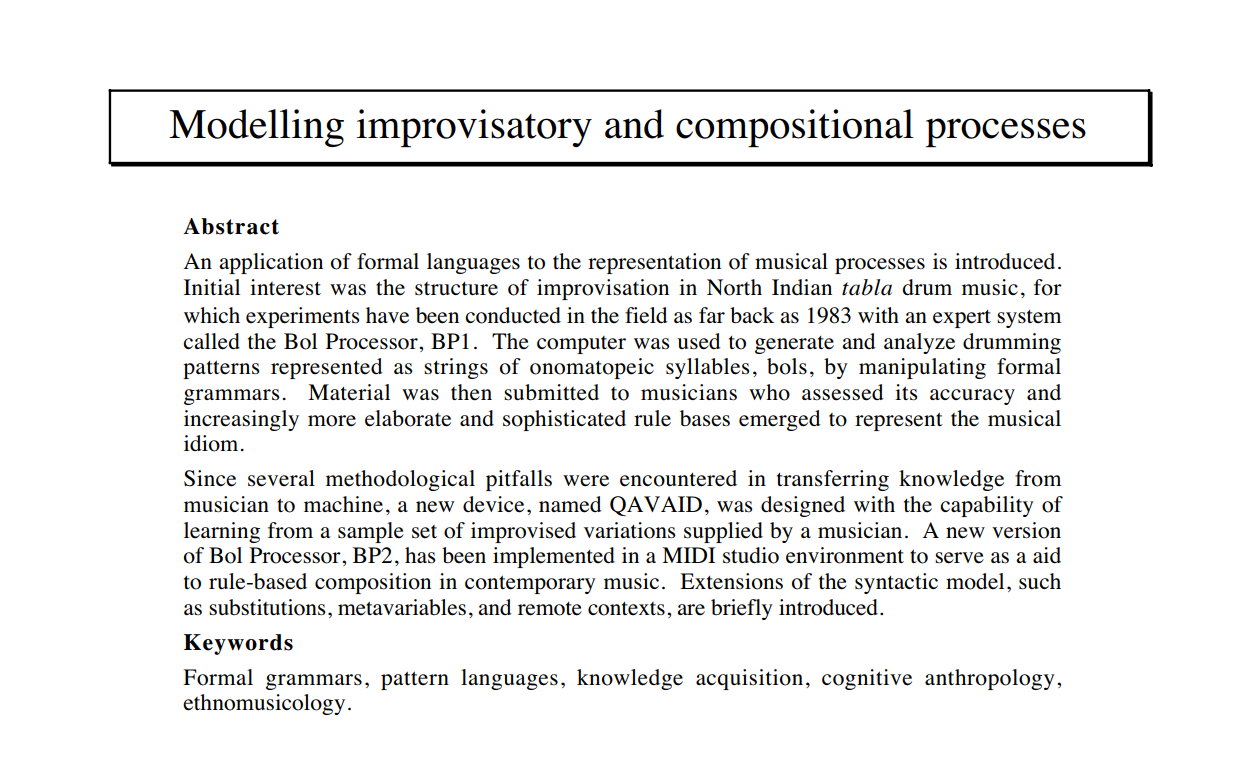
\includegraphics[keepaspectratio=true,height=.5\paperheight]{source-r.png}
\end{frame}

\begin{frame}{Grammar Symbols: Rhythmic Syllables}
\begin{hs}\begin{hscode}\SaveRestoreHook
\column{B}{@{}>{\hspre}l<{\hspost}@{}}%
\column{3}{@{}>{\hspre}l<{\hspost}@{}}%
\column{6}{@{}>{\hspre}l<{\hspost}@{}}%
\column{10}{@{}>{\hspre}l<{\hspost}@{}}%
\column{11}{@{}>{\hspre}l<{\hspost}@{}}%
\column{16}{@{}>{\hspre}l<{\hspost}@{}}%
\column{18}{@{}>{\hspre}l<{\hspost}@{}}%
\column{24}{@{}>{\hspre}l<{\hspost}@{}}%
\column{25}{@{}>{\hspre}l<{\hspost}@{}}%
\column{31}{@{}>{\hspre}l<{\hspost}@{}}%
\column{32}{@{}>{\hspre}l<{\hspost}@{}}%
\column{38}{@{}>{\hspre}l<{\hspost}@{}}%
\column{39}{@{}>{\hspre}l<{\hspost}@{}}%
\column{46}{@{}>{\hspre}l<{\hspost}@{}}%
\column{53}{@{}>{\hspre}l<{\hspost}@{}}%
\column{E}{@{}>{\hspre}l<{\hspost}@{}}%
\>[B]{}\HSKeyword{data}\;\HSCon{Syllable}{}\<[E]%
\\
\>[B]{}\hsindent{3}{}\<[3]%
\>[3]{}\HSSym{\mathrel{=}}{}\<[6]%
\>[6]{}\HSComment{ -\! - terminals}{}\<[E]%
\\
\>[6]{}\HSCon{Tr}{}\<[10]%
\>[10]{}\HSSym{\mathbin{\mid}}\HSCon{Kt}{}\<[16]%
\>[16]{}\HSSym{\mathbin{\mid}}\HSCon{Dhee}{}\<[24]%
\>[24]{}\HSSym{\mathbin{\mid}}\HSCon{Tee}{}\<[31]%
\>[31]{}\HSSym{\mathbin{\mid}}\HSCon{Dha}{}\<[38]%
\>[38]{}\HSSym{\mathbin{\mid}}\HSCon{Ta}{}\<[E]%
\\
\>[B]{}\hsindent{3}{}\<[3]%
\>[3]{}\HSSym{\mathbin{\mid}}{}\<[6]%
\>[6]{}\HSCon{Ti}{}\<[10]%
\>[10]{}\HSSym{\mathbin{\mid}}\HSCon{Ge}{}\<[16]%
\>[16]{}\HSSym{\mathbin{\mid}}\HSCon{Ke}{}\<[24]%
\>[24]{}\HSSym{\mathbin{\mid}}\HSCon{Na}{}\<[31]%
\>[31]{}\HSSym{\mathbin{\mid}}\HSCon{Ra}{}\<[38]%
\>[38]{}\HSSym{\mathbin{\mid}}\HSCon{Noop}{}\<[E]%
\\
\>[6]{}\HSComment{ -\! - non-terminals}{}\<[E]%
\\
\>[B]{}\hsindent{3}{}\<[3]%
\>[3]{}\HSSym{\mathbin{\mid}}{}\<[6]%
\>[6]{}\HSCon{S}{}\<[11]%
\>[11]{}\HSSym{\mathbin{\mid}}\HSCon{XI}{}\<[18]%
\>[18]{}\HSSym{\mathbin{\mid}}\HSCon{XD}{}\<[25]%
\>[25]{}\HSSym{\mathbin{\mid}}\HSCon{XJ}{}\<[32]%
\>[32]{}\HSSym{\mathbin{\mid}}\HSCon{XA}{}\<[39]%
\>[39]{}\HSSym{\mathbin{\mid}}\HSCon{XB}{}\<[46]%
\>[46]{}\HSSym{\mathbin{\mid}}\HSCon{XG}{}\<[53]%
\>[53]{}\HSSym{\mathbin{\mid}}\HSCon{XH}\HSSym{\mathbin{\mid}}\HSCon{XC}{}\<[E]%
\\
\>[B]{}\hsindent{3}{}\<[3]%
\>[3]{}\HSSym{\mathbin{\mid}}{}\<[6]%
\>[6]{}\HSCon{XE}{}\<[11]%
\>[11]{}\HSSym{\mathbin{\mid}}\HSCon{XF}{}\<[18]%
\>[18]{}\HSSym{\mathbin{\mid}}\HSCon{TA7}{}\<[25]%
\>[25]{}\HSSym{\mathbin{\mid}}\HSCon{TC2}{}\<[32]%
\>[32]{}\HSSym{\mathbin{\mid}}\HSCon{TE1}{}\<[39]%
\>[39]{}\HSSym{\mathbin{\mid}}\HSCon{TF1}{}\<[46]%
\>[46]{}\HSSym{\mathbin{\mid}}\HSCon{TF4}{}\<[53]%
\>[53]{}\HSSym{\mathbin{\mid}}\HSCon{TD1}{}\<[E]%
\\
\>[B]{}\hsindent{3}{}\<[3]%
\>[3]{}\HSSym{\mathbin{\mid}}{}\<[6]%
\>[6]{}\HSCon{TB2}{}\<[11]%
\>[11]{}\HSSym{\mathbin{\mid}}\HSCon{TE4}{}\<[18]%
\>[18]{}\HSSym{\mathbin{\mid}}\HSCon{TC1}{}\<[25]%
\>[25]{}\HSSym{\mathbin{\mid}}\HSCon{TB3}{}\<[32]%
\>[32]{}\HSSym{\mathbin{\mid}}\HSCon{TA8}{}\<[39]%
\>[39]{}\HSSym{\mathbin{\mid}}\HSCon{TA3}{}\<[46]%
\>[46]{}\HSSym{\mathbin{\mid}}\HSCon{TB1}{}\<[53]%
\>[53]{}\HSSym{\mathbin{\mid}}\HSCon{TA1}{}\<[E]%
\\
\>[B]{}\hsindent{3}{}\<[3]%
\>[3]{}\HSKeyword{deriving}\;\HSCon{Eq}{}\<[E]%
\\
\>[B]{}\vspace{5pt}{}\<[E]%
\\
\>[B]{}\HSSpecial{(}\HSCon{\mathbin{\twoheadrightarrow}}\HSSpecial{)}\HSSym{::}\HSVar{a}\HSSym{\to} \HSSpecial{[\mskip1.5mu }\HSVar{a}\HSSpecial{\mskip1.5mu]}\HSSym{\to} \HSCon{Rule}\;\HSVar{meta}\;\HSVar{a}{}\<[E]%
\\
\>[B]{}\HSVar{x}\HSCon{\mathbin{\twoheadrightarrow}}\HSVar{xs}\HSSym{\mathrel{=}}\HSSpecial{(}\HSVar{x}\HSSpecial{,}\HSNumeral{1}\HSSpecial{,}\HSVar{always}\HSSpecial{)}\HSCon{\mathbin{\rightarrowtriangle}}\HSVar{fold1}\HSCon{\mathbin{\ \otimes\ }}\HSSpecial{(}\HSSpecial{(}\HSSym{:\ }\HSVar{en}\HSSpecial{)}\HSSym{\mathbin{\langle\$\rangle}}\HSVar{xs}\HSSpecial{)}{}\<[E]%
\ColumnHook
\end{hscode}\resethooks
\end{hs}
\end{frame}

\begin{frame}{Grammar for Tabla Improvisation}
\savecolumns
\begin{hs}\begin{hscode}\SaveRestoreHook
\column{B}{@{}>{\hspre}l<{\hspost}@{}}%
\column{3}{@{}>{\hspre}l<{\hspost}@{}}%
\column{10}{@{}>{\hspre}c<{\hspost}@{}}%
\column{10E}{@{}l@{}}%
\column{16}{@{}>{\hspre}l<{\hspost}@{}}%
\column{27}{@{}>{\hspre}l<{\hspost}@{}}%
\column{34}{@{}>{\hspre}c<{\hspost}@{}}%
\column{34E}{@{}l@{}}%
\column{40}{@{}>{\hspre}l<{\hspost}@{}}%
\column{E}{@{}>{\hspre}l<{\hspost}@{}}%
\>[B]{}\HSVar{rhythm}\HSSym{::}\HSCon{Grammar}\;\HSSpecial{(}\HSSpecial{)}\;\HSCon{Syllable}{}\<[E]%
\\
\>[B]{}\HSVar{rhythm}\HSSym{\mathrel{=}}\HSCon{S}\HSCon{\mathbin{\ |\!:}}{}\<[E]%
\\
\>[B]{}\hsindent{3}{}\<[3]%
\>[3]{}\HSSpecial{[\mskip1.5mu }\HSCon{S}{}\<[10]%
\>[10]{}\HSCon{\mathbin{\twoheadrightarrow}}{}\<[10E]%
\>[16]{}\HSSpecial{[\mskip1.5mu }\HSCon{TE1}\HSSpecial{,}\HSCon{XI}\HSSpecial{\mskip1.5mu]}{}\<[E]%
\\
\>[B]{}\hsindent{3}{}\<[3]%
\>[3]{}\HSSpecial{,}\HSCon{XI}{}\<[10]%
\>[10]{}\HSCon{\mathbin{\twoheadrightarrow}}{}\<[10E]%
\>[16]{}\HSSpecial{[\mskip1.5mu }\HSCon{TA7}\HSSpecial{,}\HSCon{XD}\HSSpecial{\mskip1.5mu]}{}\<[27]%
\>[27]{}\HSSpecial{,}\HSCon{XD}{}\<[34]%
\>[34]{}\HSCon{\mathbin{\twoheadrightarrow}}{}\<[34E]%
\>[40]{}\HSSpecial{[\mskip1.5mu }\HSCon{TA8}\HSSpecial{\mskip1.5mu]}{}\<[E]%
\\
\>[B]{}\hsindent{3}{}\<[3]%
\>[3]{}\HSSpecial{,}\HSCon{XI}{}\<[10]%
\>[10]{}\HSCon{\mathbin{\twoheadrightarrow}}{}\<[10E]%
\>[16]{}\HSSpecial{[\mskip1.5mu }\HSCon{TF1}\HSSpecial{,}\HSCon{XJ}\HSSpecial{\mskip1.5mu]}{}\<[27]%
\>[27]{}\HSSpecial{,}\HSCon{XJ}{}\<[34]%
\>[34]{}\HSCon{\mathbin{\twoheadrightarrow}}{}\<[34E]%
\>[40]{}\HSSpecial{[\mskip1.5mu }\HSCon{TC2}\HSSpecial{,}\HSCon{XA}\HSSpecial{\mskip1.5mu]}{}\<[E]%
\\
\>[B]{}\hsindent{3}{}\<[3]%
\>[3]{}\HSSpecial{,}\HSCon{XA}{}\<[10]%
\>[10]{}\HSCon{\mathbin{\twoheadrightarrow}}{}\<[10E]%
\>[16]{}\HSSpecial{[\mskip1.5mu }\HSCon{TA1}\HSSpecial{,}\HSCon{XB}\HSSpecial{\mskip1.5mu]}{}\<[27]%
\>[27]{}\HSSpecial{,}\HSCon{XB}{}\<[34]%
\>[34]{}\HSCon{\mathbin{\twoheadrightarrow}}{}\<[34E]%
\>[40]{}\HSSpecial{[\mskip1.5mu }\HSCon{TB3}\HSSpecial{,}\HSCon{XD}\HSSpecial{\mskip1.5mu]}{}\<[E]%
\\
\>[B]{}\hsindent{3}{}\<[3]%
\>[3]{}\HSSpecial{,}\HSCon{XI}{}\<[10]%
\>[10]{}\HSCon{\mathbin{\twoheadrightarrow}}{}\<[10E]%
\>[16]{}\HSSpecial{[\mskip1.5mu }\HSCon{TF1}\HSSpecial{,}\HSCon{XG}\HSSpecial{\mskip1.5mu]}{}\<[27]%
\>[27]{}\HSSpecial{,}\HSCon{XG}{}\<[34]%
\>[34]{}\HSCon{\mathbin{\twoheadrightarrow}}{}\<[34E]%
\>[40]{}\HSSpecial{[\mskip1.5mu }\HSCon{TB2}\HSSpecial{,}\HSCon{XA}\HSSpecial{\mskip1.5mu]}{}\<[E]%
\\
\>[B]{}\hsindent{3}{}\<[3]%
\>[3]{}\HSSpecial{,}\HSCon{S}{}\<[10]%
\>[10]{}\HSCon{\mathbin{\twoheadrightarrow}}{}\<[10E]%
\>[16]{}\HSSpecial{[\mskip1.5mu }\HSCon{TA1}\HSSpecial{,}\HSCon{XH}\HSSpecial{\mskip1.5mu]}{}\<[E]%
\\
\>[B]{}\hsindent{3}{}\<[3]%
\>[3]{}\HSSpecial{,}\HSCon{XH}{}\<[10]%
\>[10]{}\HSCon{\mathbin{\twoheadrightarrow}}{}\<[10E]%
\>[16]{}\HSSpecial{[\mskip1.5mu }\HSCon{TF4}\HSSpecial{,}\HSCon{XB}\HSSpecial{\mskip1.5mu]}{}\<[27]%
\>[27]{}\HSSpecial{,}\HSCon{XH}{}\<[34]%
\>[34]{}\HSCon{\mathbin{\twoheadrightarrow}}{}\<[34E]%
\>[40]{}\HSSpecial{[\mskip1.5mu }\HSCon{TA3}\HSSpecial{,}\HSCon{XC}\HSSpecial{\mskip1.5mu]}{}\<[E]%
\\
\>[B]{}\hsindent{3}{}\<[3]%
\>[3]{}\HSSpecial{,}\HSCon{XC}{}\<[10]%
\>[10]{}\HSCon{\mathbin{\twoheadrightarrow}}{}\<[10E]%
\>[16]{}\HSSpecial{[\mskip1.5mu }\HSCon{TE4}\HSSpecial{,}\HSCon{XD}\HSSpecial{\mskip1.5mu]}{}\<[27]%
\>[27]{}\HSSpecial{,}\HSCon{XC}{}\<[34]%
\>[34]{}\HSCon{\mathbin{\twoheadrightarrow}}{}\<[34E]%
\>[40]{}\HSSpecial{[\mskip1.5mu }\HSCon{TA3}\HSSpecial{,}\HSCon{XE}\HSSpecial{\mskip1.5mu]}{}\<[E]%
\\
\>[B]{}\hsindent{3}{}\<[3]%
\>[3]{}\HSSpecial{,}\HSCon{XE}{}\<[10]%
\>[10]{}\HSCon{\mathbin{\twoheadrightarrow}}{}\<[10E]%
\>[16]{}\HSSpecial{[\mskip1.5mu }\HSCon{TA1}\HSSpecial{,}\HSCon{XD}\HSSpecial{\mskip1.5mu]}{}\<[27]%
\>[27]{}\HSSpecial{,}\HSCon{XE}{}\<[34]%
\>[34]{}\HSCon{\mathbin{\twoheadrightarrow}}{}\<[34E]%
\>[40]{}\HSSpecial{[\mskip1.5mu }\HSCon{TC1}\HSSpecial{,}\HSCon{XD}\HSSpecial{\mskip1.5mu]}{}\<[E]%
\\
\>[B]{}\hsindent{3}{}\<[3]%
\>[3]{}\HSSpecial{,}\HSCon{XC}{}\<[10]%
\>[10]{}\HSCon{\mathbin{\twoheadrightarrow}}{}\<[10E]%
\>[16]{}\HSSpecial{[\mskip1.5mu }\HSCon{TB1}\HSSpecial{,}\HSCon{XB}\HSSpecial{\mskip1.5mu]}{}\<[E]%
\\
\>[B]{}\hsindent{3}{}\<[3]%
\>[3]{}\HSSpecial{,}\HSCon{S}{}\<[10]%
\>[10]{}\HSCon{\mathbin{\twoheadrightarrow}}{}\<[10E]%
\>[16]{}\HSSpecial{[\mskip1.5mu }\HSCon{TB1}\HSSpecial{,}\HSCon{XF}\HSSpecial{\mskip1.5mu]}{}\<[E]%
\\
\>[B]{}\hsindent{3}{}\<[3]%
\>[3]{}\HSSpecial{,}\HSCon{XF}{}\<[10]%
\>[10]{}\HSCon{\mathbin{\twoheadrightarrow}}{}\<[10E]%
\>[16]{}\HSSpecial{[\mskip1.5mu }\HSCon{TA1}\HSSpecial{,}\HSCon{XJ}\HSSpecial{\mskip1.5mu]}{}\<[27]%
\>[27]{}\HSSpecial{,}\HSCon{XF}{}\<[34]%
\>[34]{}\HSCon{\mathbin{\twoheadrightarrow}}{}\<[34E]%
\>[40]{}\HSSpecial{[\mskip1.5mu }\HSCon{TD1}\HSSpecial{,}\HSCon{XG}\HSSpecial{\mskip1.5mu]}{}\<[E]%
\ColumnHook
\end{hscode}\resethooks
\end{hs}
\end{frame}

\begin{frame}{Grammar for Tabla Improvisation}
\restorecolumns
\begin{hs}\begin{hscode}\SaveRestoreHook
\column{B}{@{}>{\hspre}l<{\hspost}@{}}%
\column{3}{@{}>{\hspre}l<{\hspost}@{}}%
\column{10}{@{}>{\hspre}c<{\hspost}@{}}%
\column{10E}{@{}l@{}}%
\column{16}{@{}>{\hspre}l<{\hspost}@{}}%
\column{E}{@{}>{\hspre}l<{\hspost}@{}}%
\>[3]{}\HSSpecial{,}\HSCon{TA7}{}\<[10]%
\>[10]{}\HSCon{\mathbin{\twoheadrightarrow}}{}\<[10E]%
\>[16]{}\HSSpecial{[\mskip1.5mu }\HSCon{Kt}\HSSpecial{,}\HSCon{Dha}\HSSpecial{,}\HSCon{Tr}\HSSpecial{,}\HSCon{Kt}\HSSpecial{,}\HSCon{Dha}\HSSpecial{,}\HSCon{Ge}\HSSpecial{,}\HSCon{Na}\HSSpecial{\mskip1.5mu]}{}\<[E]%
\\
\>[3]{}\HSSpecial{,}\HSCon{TC2}{}\<[10]%
\>[10]{}\HSCon{\mathbin{\twoheadrightarrow}}{}\<[10E]%
\>[16]{}\HSSpecial{[\mskip1.5mu }\HSCon{Tr}\HSSpecial{,}\HSCon{Kt}\HSSpecial{\mskip1.5mu]}\HSSpecial{,}\;\HSCon{TE1}\HSCon{\mathbin{\twoheadrightarrow}}\HSSpecial{[\mskip1.5mu }\HSCon{Tr}\HSSpecial{\mskip1.5mu]}\HSSpecial{,}\;\HSCon{TF1}\HSCon{\mathbin{\twoheadrightarrow}}\HSSpecial{[\mskip1.5mu }\HSCon{Kt}\HSSpecial{\mskip1.5mu]}{}\<[E]%
\\
\>[3]{}\HSSpecial{,}\HSCon{TF4}{}\<[10]%
\>[10]{}\HSCon{\mathbin{\twoheadrightarrow}}{}\<[10E]%
\>[16]{}\HSSpecial{[\mskip1.5mu }\HSCon{Ti}\HSSpecial{,}\HSCon{Dha}\HSSpecial{,}\HSCon{Tr}\HSSpecial{,}\HSCon{Kt}\HSSpecial{\mskip1.5mu]}{}\<[E]%
\\
\>[3]{}\HSSpecial{,}\HSCon{TE4}{}\<[10]%
\>[10]{}\HSCon{\mathbin{\twoheadrightarrow}}{}\<[10E]%
\>[16]{}\HSSpecial{[\mskip1.5mu }\HSCon{Ti}\HSSpecial{,}\HSCon{Noop}\HSSpecial{,}\HSCon{Dha}\HSSpecial{,}\HSCon{Ti}\HSSpecial{\mskip1.5mu]}{}\<[E]%
\\
\>[3]{}\HSSpecial{,}\HSCon{TD1}{}\<[10]%
\>[10]{}\HSCon{\mathbin{\twoheadrightarrow}}{}\<[10E]%
\>[16]{}\HSSpecial{[\mskip1.5mu }\HSCon{Noop}\HSSpecial{\mskip1.5mu]}\HSSpecial{,}\;\HSCon{TB2}\HSCon{\mathbin{\twoheadrightarrow}}\HSSpecial{[\mskip1.5mu }\HSCon{Dha}\HSSpecial{,}\HSCon{Ti}\HSSpecial{\mskip1.5mu]}\HSSpecial{,}\;\HSCon{TC1}\HSCon{\mathbin{\twoheadrightarrow}}\HSSpecial{[\mskip1.5mu }\HSCon{Ge}\HSSpecial{\mskip1.5mu]}{}\<[E]%
\\
\>[3]{}\HSSpecial{,}\HSCon{TB3}{}\<[10]%
\>[10]{}\HSCon{\mathbin{\twoheadrightarrow}}{}\<[10E]%
\>[16]{}\HSSpecial{[\mskip1.5mu }\HSCon{Dha}\HSSpecial{,}\HSCon{Tr}\HSSpecial{,}\HSCon{Kt}\HSSpecial{\mskip1.5mu]}{}\<[E]%
\\
\>[3]{}\HSSpecial{,}\HSCon{TA8}{}\<[10]%
\>[10]{}\HSCon{\mathbin{\twoheadrightarrow}}{}\<[10E]%
\>[16]{}\HSSpecial{[\mskip1.5mu }\HSCon{Dha}\HSSpecial{,}\HSCon{Ti}\HSSpecial{,}\HSCon{Dha}\HSSpecial{,}\HSCon{Ge}\HSSpecial{,}\HSCon{Dhee}\HSSpecial{,}\HSCon{Na}\HSSpecial{,}\HSCon{Ge}\HSSpecial{,}\HSCon{Na}\HSSpecial{\mskip1.5mu]}{}\<[E]%
\\
\>[3]{}\HSSpecial{,}\HSCon{TA3}{}\<[10]%
\>[10]{}\HSCon{\mathbin{\twoheadrightarrow}}{}\<[10E]%
\>[16]{}\HSSpecial{[\mskip1.5mu }\HSCon{Tr}\HSSpecial{,}\HSCon{Kt}\HSSpecial{,}\HSCon{Dha}\HSSpecial{\mskip1.5mu]}\HSSpecial{,}\HSCon{TB1}\HSCon{\mathbin{\twoheadrightarrow}}\HSSpecial{[\mskip1.5mu }\HSCon{Ti}\HSSpecial{\mskip1.5mu]}\HSSpecial{,}\HSCon{TA1}\HSCon{\mathbin{\twoheadrightarrow}}\HSSpecial{[\mskip1.5mu }\HSCon{Dha}\HSSpecial{\mskip1.5mu]}\;\HSSpecial{\mskip1.5mu]}{}\<[E]%
\ColumnHook
\end{hscode}\resethooks
\end{hs}
\end{frame}

\begin{frame}{Interpretation: From Syllables to MIDI}
\begin{hs}\begin{hscode}\SaveRestoreHook
\column{B}{@{}>{\hspre}l<{\hspost}@{}}%
\column{3}{@{}>{\hspre}l<{\hspost}@{}}%
\column{5}{@{}>{\hspre}l<{\hspost}@{}}%
\column{7}{@{}>{\hspre}l<{\hspost}@{}}%
\column{36}{@{}>{\hspre}l<{\hspost}@{}}%
\column{E}{@{}>{\hspre}l<{\hspost}@{}}%
\>[B]{}\HSKeyword{instance}\;\HSCon{ToMusic1}\;\HSCon{Syllable}\;\HSKeyword{where}{}\<[E]%
\\
\>[B]{}\hsindent{3}{}\<[3]%
\>[3]{}\HSVar{toMusic1}\HSSym{\mathrel{=}}\HSVar{toMusic}\HSSym{\mathbin{\circ}}\HSVar{pitch}\HSSym{\mathbin{\circ}}\HSVar{percussionMap}{}\<[E]%
\\
\>[3]{}\hsindent{2}{}\<[5]%
\>[5]{}\HSKeyword{where}{}\<[E]%
\\
\>[5]{}\hsindent{2}{}\<[7]%
\>[7]{}\HSVar{percussionMap}\HSSym{::}\HSCon{Syllable}\HSSym{\to} \HSCon{Int}{}\<[E]%
\\
\>[5]{}\hsindent{2}{}\<[7]%
\>[7]{}\HSVar{percussionMap}\;\HSVar{s}\HSSym{\mathrel{=}}\HSKeyword{case}\;\HSVar{s}\;\HSKeyword{of}\;{}\<[36]%
\>[36]{}\HSCon{Tr}\HSSym{\to} \HSNumeral{38}{}\<[E]%
\\
\>[36]{}\HSCon{Kt}\HSSym{\to} \HSNumeral{45}{}\<[E]%
\\
\>[36]{}\HSSym{\dots}{}\<[E]%
\ColumnHook
\end{hscode}\resethooks
\end{hs}
\end{frame}
\section{Generated Results}

\begin{frame}{Songs as Configurations}
\begin{itemize}
\item Given a total duration and the required configurations, generate a "music piece":
\begin{hs}\begin{hscode}\SaveRestoreHook
\column{B}{@{}>{\hspre}l<{\hspost}@{}}%
\column{3}{@{}>{\hspre}l<{\hspost}@{}}%
\column{11}{@{}>{\hspre}c<{\hspost}@{}}%
\column{11E}{@{}l@{}}%
\column{13}{@{}>{\hspre}l<{\hspost}@{}}%
\column{15}{@{}>{\hspre}l<{\hspost}@{}}%
\column{19}{@{}>{\hspre}l<{\hspost}@{}}%
\column{E}{@{}>{\hspre}l<{\hspost}@{}}%
\>[B]{}\HSVar{generate}{}\<[11]%
\>[11]{}\HSSym{::}{}\<[11E]%
\>[15]{}\HSCon{FilePath}\HSSym{\to} \HSCon{Dur}{}\<[E]%
\\
\>[11]{}\HSSym{\to} {}\<[11E]%
\>[15]{}\HSCon{HarmonyConfig}\HSSym{\to} \HSCon{MelodyConfig}{}\<[E]%
\\
\>[11]{}\HSSym{\to} {}\<[11E]%
\>[15]{}\HSCon{IO}\;\HSSpecial{(}\HSSpecial{)}{}\<[E]%
\\
\>[B]{}\HSVar{generate}\;\HSVar{f}\;\HSVar{t}\;\HSVar{hCfg}\;\HSVar{mCfg}\HSSym{\mathrel{=}}\HSKeyword{do}{}\<[E]%
\\
\>[B]{}\hsindent{3}{}\<[3]%
\>[3]{}\HSSpecial{(}\HSVar{absHarm}\HSSpecial{,}\HSVar{harm}\HSSpecial{)}\HSSym{\leftarrow} \HSVar{runGrammar}\;\HSVar{harmony}\;\HSVar{t}\;\HSVar{hCfg}{}\<[E]%
\\
\>[B]{}\hsindent{3}{}\<[3]%
\>[3]{}\HSSpecial{(}\HSSym{\anonymous} \HSSpecial{,}{}\<[13]%
\>[13]{}\HSVar{mel}\HSSpecial{)}{}\<[19]%
\>[19]{}\HSSym{\leftarrow} \HSVar{runGrammar}\;\HSVar{melody}\;\HSVar{t}\;\HSSpecial{(}\HSVar{mCfg}\HSSpecial{,}\HSVar{absHarm}\HSSpecial{)}{}\<[E]%
\\
\>[B]{}\hsindent{3}{}\<[3]%
\>[3]{}\HSSpecial{(}\HSSym{\anonymous} \HSSpecial{,}{}\<[13]%
\>[13]{}\HSVar{rhy}\HSSpecial{)}{}\<[19]%
\>[19]{}\HSSym{\leftarrow} \HSVar{runGrammar}\;\HSVar{rhythm}\;\HSVar{t}\;\HSSpecial{(}\HSSpecial{)}{}\<[E]%
\\
\>[B]{}\hsindent{3}{}\<[3]%
\>[3]{}\HSVar{writeToMidiFile}\;\HSVar{f}\;\HSSpecial{(}\HSVar{harm}\HSCon{\mathbin{:=:}}\HSVar{mel}\HSCon{\mathbin{:=:}}\HSVar{rhy}\HSSpecial{)}{}\<[E]%
\ColumnHook
\end{hscode}\resethooks
\end{hs}
\end{itemize}
\end{frame}

\begin{frame}{Sonata in E Minor}
\begin{hs}\begin{hscode}\SaveRestoreHook
\column{B}{@{}>{\hspre}l<{\hspost}@{}}%
\column{5}{@{}>{\hspre}l<{\hspost}@{}}%
\column{7}{@{}>{\hspre}l<{\hspost}@{}}%
\column{18}{@{}>{\hspre}l<{\hspost}@{}}%
\column{20}{@{}>{\hspre}l<{\hspost}@{}}%
\column{E}{@{}>{\hspre}l<{\hspost}@{}}%
\>[B]{}\HSVar{sonata}{}\<[E]%
\\
\>[B]{}\HSSym{\mathrel{=}}{}\<[5]%
\>[5]{}\HSVar{generate}\;\HSString{``sonata\char34 }\;\HSSpecial{(}\HSNumeral{12}\HSSym{*}\HSVar{wn}\HSSpecial{)}{}\<[E]%
\\
\>[5]{}\HSCon{HarmonyConfig}\;{}\<[E]%
\\
\>[5]{}\hsindent{2}{}\<[7]%
\>[7]{}\HSSpecial{\{\mskip1.5mu }\HSVar{basePc}{}\<[20]%
\>[20]{}\HSSym{\mathrel{=}}\HSCon{E}{}\<[E]%
\\
\>[5]{}\hsindent{2}{}\<[7]%
\>[7]{}\HSSpecial{,}\HSVar{baseOct}{}\<[20]%
\>[20]{}\HSSym{\mathrel{=}}\HSNumeral{4}{}\<[E]%
\\
\>[5]{}\hsindent{2}{}\<[7]%
\>[7]{}\HSSpecial{,}\HSVar{baseScale}{}\<[20]%
\>[20]{}\HSSym{\mathrel{=}}\HSVar{minor}{}\<[E]%
\\
\>[5]{}\hsindent{2}{}\<[7]%
\>[7]{}\HSSpecial{,}\HSVar{chords}{}\<[20]%
\>[20]{}\HSSym{\mathrel{=}}\HSVar{equally}\;\HSSpecial{[\mskip1.5mu }\HSVar{mi}\HSSpecial{,}\HSVar{maj}\HSSpecial{,}\HSVar{dim}\HSSpecial{\mskip1.5mu]}\HSSpecial{\mskip1.5mu\}}{}\<[E]%
\\
\>[5]{}\HSCon{MelodyConfig}\;{}\<[E]%
\\
\>[5]{}\hsindent{2}{}\<[7]%
\>[7]{}\HSSpecial{\{\mskip1.5mu }\HSVar{scales}{}\<[18]%
\>[18]{}\HSSym{\mathrel{=}}\HSVar{equally}\;\HSSpecial{[\mskip1.5mu }\HSVar{ionian}\HSSpecial{,}\HSVar{harmonicMinor}\HSSpecial{\mskip1.5mu]}{}\<[E]%
\\
\>[5]{}\hsindent{2}{}\<[7]%
\>[7]{}\HSSpecial{,}\HSVar{octaves}{}\<[18]%
\>[18]{}\HSSym{\mathrel{=}}\HSSpecial{[\mskip1.5mu }\HSSpecial{(}\HSNumeral{5}\HSSpecial{,}\HSNumeral{4}\HSSpecial{)}\HSSpecial{,}\HSSpecial{(}\HSNumeral{20}\HSSpecial{,}\HSNumeral{5}\HSSpecial{)}\HSSpecial{,}\HSSpecial{(}\HSNumeral{10}\HSSpecial{,}\HSNumeral{6}\HSSpecial{)}\HSSpecial{\mskip1.5mu]}\HSSpecial{\mskip1.5mu\}}{}\<[E]%
\ColumnHook
\end{hscode}\resethooks
\end{hs}
\end{frame}

\begin{frame}{Oriental Algebras}
\begin{hs}\begin{hscode}\SaveRestoreHook
\column{B}{@{}>{\hspre}l<{\hspost}@{}}%
\column{5}{@{}>{\hspre}l<{\hspost}@{}}%
\column{7}{@{}>{\hspre}l<{\hspost}@{}}%
\column{18}{@{}>{\hspre}l<{\hspost}@{}}%
\column{20}{@{}>{\hspre}l<{\hspost}@{}}%
\column{E}{@{}>{\hspre}l<{\hspost}@{}}%
\>[B]{}\HSVar{orientalAlgebras}{}\<[E]%
\\
\>[B]{}\HSSym{\mathrel{=}}{}\<[5]%
\>[5]{}\HSVar{generate}\;\HSString{``oriental\char34 }\;\HSSpecial{(}\HSNumeral{12}\HSSym{*}\HSVar{wn}\HSSpecial{)}{}\<[E]%
\\
\>[5]{}\HSCon{HarmonyConfig}\;{}\<[E]%
\\
\>[5]{}\hsindent{2}{}\<[7]%
\>[7]{}\HSSpecial{\{\mskip1.5mu }\HSVar{basePc}{}\<[20]%
\>[20]{}\HSSym{\mathrel{=}}\HSCon{A}{}\<[E]%
\\
\>[5]{}\hsindent{2}{}\<[7]%
\>[7]{}\HSSpecial{,}\HSVar{baseOct}{}\<[20]%
\>[20]{}\HSSym{\mathrel{=}}\HSNumeral{3}{}\<[E]%
\\
\>[5]{}\hsindent{2}{}\<[7]%
\>[7]{}\HSSpecial{,}\HSVar{baseScale}{}\<[20]%
\>[20]{}\HSSym{\mathrel{=}}\HSVar{arabian}\HSComment{ -\! - $\equiv$ [P1, M2, Mi3, P4, A4, Mi6, M7]}{}\<[E]%
\\
\>[5]{}\hsindent{2}{}\<[7]%
\>[7]{}\HSSpecial{,}\HSVar{chords}{}\<[20]%
\>[20]{}\HSSym{\mathrel{=}}\HSVar{equally}\;\HSVar{allChords}\HSSpecial{\mskip1.5mu\}}{}\<[E]%
\\
\>[5]{}\HSCon{MelodyConfig}\;{}\<[E]%
\\
\>[5]{}\hsindent{2}{}\<[7]%
\>[7]{}\HSSpecial{\{\mskip1.5mu }\HSVar{scales}{}\<[18]%
\>[18]{}\HSSym{\mathrel{=}}\HSVar{equally}\;\HSVar{allScales}{}\<[E]%
\\
\>[5]{}\hsindent{2}{}\<[7]%
\>[7]{}\HSSpecial{,}\HSVar{octaves}{}\<[18]%
\>[18]{}\HSSym{\mathrel{=}}\HSSpecial{[\mskip1.5mu }\HSSpecial{(}\HSNumeral{20}\HSSpecial{,}\HSNumeral{4}\HSSpecial{)}\HSSpecial{,}\HSSpecial{(}\HSNumeral{15}\HSSpecial{,}\HSNumeral{5}\HSSpecial{)}\HSSpecial{,}\HSSpecial{(}\HSNumeral{5}\HSSpecial{,}\HSNumeral{6}\HSSpecial{)}\HSSpecial{\mskip1.5mu]}\HSSpecial{\mskip1.5mu\}}{}\<[E]%
\ColumnHook
\end{hscode}\resethooks
\end{hs}
\end{frame}

\section{Conclusion}

\begin{frame}{Future Work}
\begin{itemize}
\item Jazz harmony (extend with context-sensitive features)
  \begin{itemize}
  \item \textit{[Steedman, 1984]} A generative grammar for jazz chord sequences
  \item \textit{[Steedman, 1996]} The blues and the abstract truth
  \end{itemize}
\item Better \& more principled interpretation
\item Intrinsically-typed grammars
\item Non-musical Domains
\end{itemize}
\end{frame}

\begin{frame}{Conclusion}
\setlength{\epigraphwidth}{.5\linewidth}
\epigraph{\textit{It's gotta be simple, so people can dig it!}}{Thelonious Monk}
\end{frame}

\begin{frame}[standout]
  Questions?
\end{frame}

\end{document}
